
%%%%%%%%%%%%%%%%%%%%%%%%%%%%%%%%%%%%%%%%%%%%%%%
%  TITLE
%
% (A title should be specific, informative, and brief. Use
% abbreviations only if they are defined in the abstract. Titles that
% start with general keywords then specific terms are optimized in
% searches)
%
%%%%%%%%%%%%%%%%%%%%%%%%%%%%%%%%%%%%%%%%%%%%%%%

% Example: \title{This is a test title}
\title{The biogeochemichal model data base \texttt{bgc\_md2} and python
packages  \LAPM, \CompartmentalSystems, \ComputabilityGraphs for the analysis of compartmental dynamical systems}
%\date{\today}
%%%%%%%%%%%%%%%%%%%%%%%%%%%%%%%%%%%%%%%%%%%%%%%
%
%  AUTHORS AND AFFILIATIONS
%
%%%%%%%%%%%%%%%%%%%%%%%%%%%%%%%%%%%%%%%%%%%%%%%

% Authors are individuals who have significantly contributed to the
% research and preparation of the article. Group authors are allowed, if
% each author in the group is separately identified in an appendix.)

% List authors by first name or initial followed by last name and
% separated by commas. Use \affil{} to number affiliations, and
% \thanks{} for author notes.
% Additional author notes should be indicated with \thanks{} (for
% example, for current addresses).

% Example: \authors{A. B. Author\affil{1}\thanks{Current address, Antartica}, B. C. Author\affil{2,3}, and D. E.
% Author\affil{3,4}\thanks{Also funded by Monsanto.}}

% \affiliation{1}{First Affiliation}
% \affiliation{2}{Second Affiliation}
% \affiliation{3}{Third Affiliation}
% \affiliation{4}{Fourth Affiliation}

%\affiliation{=number=}{=Affiliation Address=}
%(repeat as many times as is necessary)

\author[2]{M{arkus M{\"{u}}ller}}
\author[4]{Holger Metzler}
\author[3]{Ver{\'{o}}nika Ceballos-N{\'{u}}{\~{n}}ez}
\author[1]{Carlos A. Sierra}
\author[2]{Konstiantin Viatkin}
\author[2]{Yiqi Luo}
\affil[1]{Max Planck Institute for Biogeochemistry, Hans-Knöll-Str. 10, 07745 Jena, Germany}
\affil[2]{Cornell}
\affil[3]{}
\affil[4]{}

\begin{abstract} \noindent
  
Compartmental systems are a particular class of dynamical systems that describe
the flow of conserved quantities such as mass and energy through a network of
interconnected compartments. 
The main purpose and greatest challenge of this
work is to make such models {\bf transparent} by facilitating comparisons
between them. 
The central narrativ of this paper is the quest to implement a software tool that makes this possible. 
Uncommonly we do not start with a particular scientific question but use the mathematical rigor required by an actual implementation as a guidelind to set the possible scientific scope for model comparison.
The scientific challenge is to find the common
diagnostics by which we can compare models. The technical challenges are,
firstly to implement the diagnostics in a way that makes them applicable to all collected
models, secondly how to \emph{describe} models comparably to allow queries but flexibly enough 
to formulate them in the many different
ways in which they appear in the literature and thirdly compactly enough to facilitate a maintainable collection of reasonable size. 

We enhance the common diagnostics of pool contents and fluxes by the 
computations of age and transit time distributions for whole models and
especially subsystems like vegation or soil which is essential 
to compare models with conceptually different pools, i.e. two ecosystem models
w.r.t the vegetation part , consisting however of two pools
(i.e. leaf and root) in one but three pools (i.e. leaf, wood, root) in the
other. 
We provide an extensible, declarative domain specific language (DSL) to enable (data base) queries and reduce the amount of model specific code by orders of magnitude. 
avoiding duplication in two novel ways: It defines an extensible set of 
building blocks common to all models and implemented in symbolic math via \texttt{sympy} as special types, and an extensible set of type annotated functions operating on these types as 
building blocks which can be combined automatically by a graph library to compute every result,
reachable by any recursive combination of these functions. 
This allows us to formulate models compactly and
flexibly in different equivalent ways i.e. via fluxes, flowdiagrams, or
matrices and at the same time to avoid the implementation of many similar
functions for the same result. Thus we can also not only query and compare
what is \emph{provided}, as in the model description records of a conventional data
base, but also what is \emph{computable} from them. 

Apart from the technical aspects the rigorous description of models via a
strictly typed functional DSL also informs the choice of diagnostics variables by
excluding ambigously defined candidates that have been proposed in the literature. 
The combination of these capabilities is implemented in open source python
packages \texttt{bgc\_md2} (Biogeochemical Model Database ), 
\LAPM (Linear Autonomous Pool Models),
\CompartmentalSystems and \ComputabilityGraphs, available on GitHub and for testing even without installation on binder. 
We proof the above mentioned concepts by comparing four global land carbon models with respect to transient ages and transit times.
%implemented analysis tools include symbolic computations of model
%decomposition into subsystems, flowdiagrams, transformation and reformulation
%with respect to different building blocks e.g. matrix versus flux equations and
%also difficult to obtain numerical metrics to characterize timescales of mass
%flow in compartmental systems such as the age of the mass and transit time
%trough the entire system, subsystems like vegetation or soil, or individual
%compartments.
%The actual computations were outsourced into other packages where \LAPM (Linear
%Autonomous Pool Models) provides functions for the analysis of compartmental
%systems at equilibrium, \CompartmentalSystems tools for the analysis of
%non-autonomous linear compartmental systems and \ComputabilityGraphs
%determines the set of all possible computations that can be performed on a
%model depending on information available from its description.

\end{abstract}

\section*{Plain Language Summary} 
Imagine a bucket standing on a table under a
water tap. Now drill some small holes in the bottom and attach some short pipes
that lead to other buckets standing on some chairs and drill holes in ther
bottom to attach pipes to even more buckets standing on the ground. Drill holes
again in the bottom ...
It turns out that regardless of the number of buckets pipes or taps, the amount of water in the buckets at
any time in the future can be predicted very accurately without knowing the
details of how exactly the water flows through the buckets, for instance where
the holes in the bottom are or which path a single water molecule takes
through the bucket.  Actually it is enough to know three things: how
much water is in the buckets at the start, how much water comes out of the tap
at any time and how the outflux through the holes depends on the amount of
water in the bucket i.e. how big the holes are.  
The simplicity of this description is extremely attractive and has made bucket or pool models prolific in many
branches of science, describing, apart from the obvious physical examaples, phenomena including  chemical reactors or
ecological earth system models for the carbon cycle essential for estimating future climate change.
All these models are called \emph{compartmental models}.  
We developed a set of software tools that makes it much easier to describe, translate, collect, inspect, and ultimately compare such models.  
While the tools are as widely applicable as compartmental models, the example applications we present are inspired by our own work in the global carbon cycle where the reduction of uncertainty of model predictions is a major goal for climate change mitigation and a strong motivation for model intercomparisons and the increased transparancy facilitating them. 
Our tools can translate the simple description given above into a system of ordinary differential equations and vice versa visualize such a matrix  equationas system of interconnected buckets. They can compute complex numerical results that are comparable to physical quanteties that are actually measurable. 
The ability to do this for a large number of models, made possible by a parsimonious description, is unprecedented and makes every single model much more transparent. 
Our software tools are free to use, change and extend.
The aim of this article is to make them available to researchers who want to use them, show the way how they can be extendet but also to discuss what more fundamental lessons we have learned in the process of their creation e.g. w.r.t which criteria compartmental models should be compared.
%%%%%%%%%%%%%%%%%%%%%%%%%%%%%%%%%%%%%%%%%%%%%%%
%
%  BODY TEXT
%
%%%%%%%%%%%%%%%%%%%%%%%%%%%%%%%%%%%%%%%%%%%%%%%

%%% Suggested section heads:
% \section{Introduction}
%
% The main text should start with an introduction. Except for short
% manuscripts (such as comments and replies), the text should be divided
% into sections, each with its own heading.

% Headings should be sentence fragments and do not begin with a
% lowercase letter or number. Examples of good headings are:

% \section{Materials and Methods}
% Here is text on Materials and Methods.
%
% \subsection{A descriptive heading about methods}
% More about Methods.
%
% \section{Data} (Or section title might be a descriptive heading about data)
%
% \section{Results} (Or section title might be a descriptive heading about the
% results)
%
% \section{Conclusions}


%\section{Motivation and significance}
\section{Introduction}
The principle of mass conservation plays a central role in mathematical models
of natural systems in a variety of scientific fields such as systems biology,
toxicology, pharmacokinetics \citep{Anderson1983}, ecology
\citep{Eriksson1971ARoEaS, Rodhe1979Tellus, Matis1979, Manzoni2009SBB},
hydrology \citep{Nash1957IASH, Botter2011GRL, Harman2014GRL}, biogeochemistry
\citep{Manzoni2009SBB, Sierra2015EM}, and epidemiology \citep{Jacquez1993SIAM}.
In most cases such models are nonnegative dynamical systems that can be
described by first-order systems of ordinary differential equations (ODEs) with
strong structural constraints.  Such systems are called compartmental systems
\citep{Anderson1983, Jacquez1993SIAM, Walter1999, Haddad2010}, and have
important mathematical properties that aid in their analysis and study.

\subsection{New Diagnostics} 
As mass moves across a compartmental system, it is often of interest to study
properties of the compartments, the entire system or subsystems related to the speed at
which the mass moves, and the time it takes mass to pass through specific
paths. These properties are generally characterized
by metrics such as the \emph{age} of mass with respect to the entry to the entire
system, a subsystem, or a single compartment and the \emph{transit time} of mass 
across the entire network of compartments or parts of it until its
final exit. 
However, methods traditionally used in the literature, to compute these metrics for
compartmental systems depended on specific assumptions imposed on the system
of equations \citep{Sierra2017GCB} and restricted either the applicability 
of the procedures or the interpretability of the results if applied to situations 
where those conditions where not fulfilled exactly. 

\subsection{Origin and Present State of Software Tools}
This becomes a challenge when they are implemented in software.
It is much easier to claim that something is computable than to implement it.
It is much easier to warn a scientist to check the applicability of a method than to avoid
a misapplication of that function automatically.
It is much easier to present a proof of concept of one or two diagnostic variable for one or two models than to build and maintain a collection of many models and many diagnostics.

Over the course of more than ten years and with the help of contributions of many people we have 
developed a practically usable collection of many powerfull tools to formulate, inspect and query a collection of compartmental models, i.e. a model data base.
We have learned some hard lessons in the process. 
While coding has become a major part of science, and greatly enhances our ability of prediction, it has also obscured the ways to obtain them. 
A way to apply the \emph{same} tools to \emph{many} models is a very attractive propositon to regain some of the transparancy by well defined comparisons. 
As the number of models and the number of applicable diagnostics become more numerous the 
the number of cobinations grows bilinearly, and with it the 
technical challenges to maintain both collections.
A 'copy and paste' approach becomes unmaintainable very quickly, 
in our case deinitely before the present number of about 30+ models had been reached. 
Ideally we want to turn the bilinear growth of combinations of models and diagnostic tools 
into an advantage and make all diagnostics available to all models. 
To make this possible the right abstractions have to be found, 
just to keep the size of the code base in check. 
At the outset it is very easy to overlook that the right abstractions 
are an emerging feature and \emph{change} with the addition of more models and new methods.
To be able to repeatedly refactor the code base w.r.t better abstractions 
requires software engenering techniques like unit testing and more specifically a 
'test hull' i.e. a comprehensive set of test to provide test coverage for the features, so that their implementation can be changed with confidence.
Apart from the benefit of inducing better engeneering practices the work on a
model data base has the benefit of \emph{unveiling} these abstractions.  
Their choice is not accidental but the result of a decade of refinement and a major 
outcome of the project. 
An example for this clarifying feedback of software development to science is  
the basic requirement, to be able to  define  a result of a computation by a function implementing this computaiton.
Astonishingly this excludes some metrics for compartmental systems that have been proposed as we will see.

Our first encounter with this challenge was the development of \SoilR \citep{SoilR}, a \texttt{R} package that collects a number of compartmental models specialized on soil models.
The sofware we are going to present can be seen as the result of countless refactoring and two major design iterations of this
initial project, the result of contributions of many codevelopers, user input,  
and a decade of critical eavaluation and resulting change of design choices.
The result not only far exceeds \SoilR's 
capabilities but also constitutes our best proposal for an extendable community tool so far.
In particular the new approach
\begin{enumerate}
  \item
    is based on symbolic math, which allows users to look at models
    as they appear in publications, in the form of equations and flow diagrams,
    enables symbolic analysis (e.g. computing derivatives for sensitivity analysis)
  \item 
    describes compartmental models as graphs, or matrix equations and enables the conversions between them, thereby enableling the definition of subsystems by simply naming their pools.
  \item
    adds diagnostics (transit time and age distributions) not present in \SoilR.
  \item
    provides a much simpler user interface 
    to the vast number of analytical tools that had already made the creation of a navigatable documentation an overwhelming job for \SoilR. 

  \item
    simplifies the description of models by much smaller building blocks that are combined
    \emph{automatically}, rather than forcing the developers to implement (and a user to choose) a
    huge number of model constructing function. 
  \item 
    automatically combines functions to compute results recursively
\end{enumerate}

We developed three python packages for the representation, classification, collection and analysis  of compartmental systems, implementing methods for the computation of age and transit times, that can be performed for particular systems under given assumptions, and tools to automatically \emph{restrict} their use.
These open source packages are called: 
\LAPM (Linear Autonomous Pool Models),
\CompartmentalSystems  and
\texttt{bgc\_md2} (Biogeochemical Model Database).
This manuscript provides a general introduction to these packages 
with emphasis of their combined use via \texttt{bgc\_md2} ,
The latter implements a set of model describing properties that form the (exclusive) arguments and return values of strictly typed functions, forming a network of computability which we use 
to implement a declarative domain specific language for model creation, inspection, querying and thus comparison.
To facilitate this we implemented a fourth package \ComputabilityGraphs based upon the  type hinting syntax of modern \python versions, extendig its use to predicting what is computable.   
The requirement to define every model property as a variable of a specific type, and to provide a function to compute it from other model propertie (i.e. variable of well defined \emph{types}) also provides a rigorous filter for what constitutes a diagnostic variable. 
We use it as such to discuss why we implemented or excluded some diagnostics proposed in the literature.
Practically we use this language to create a small
(30+) collection of models, motivated by our own work on the terrestrial carbon
cycle.  Some screenshot of the software are shown in \figref{fig:overview}
\begin{figure}[h]
  \label{fig:overview}
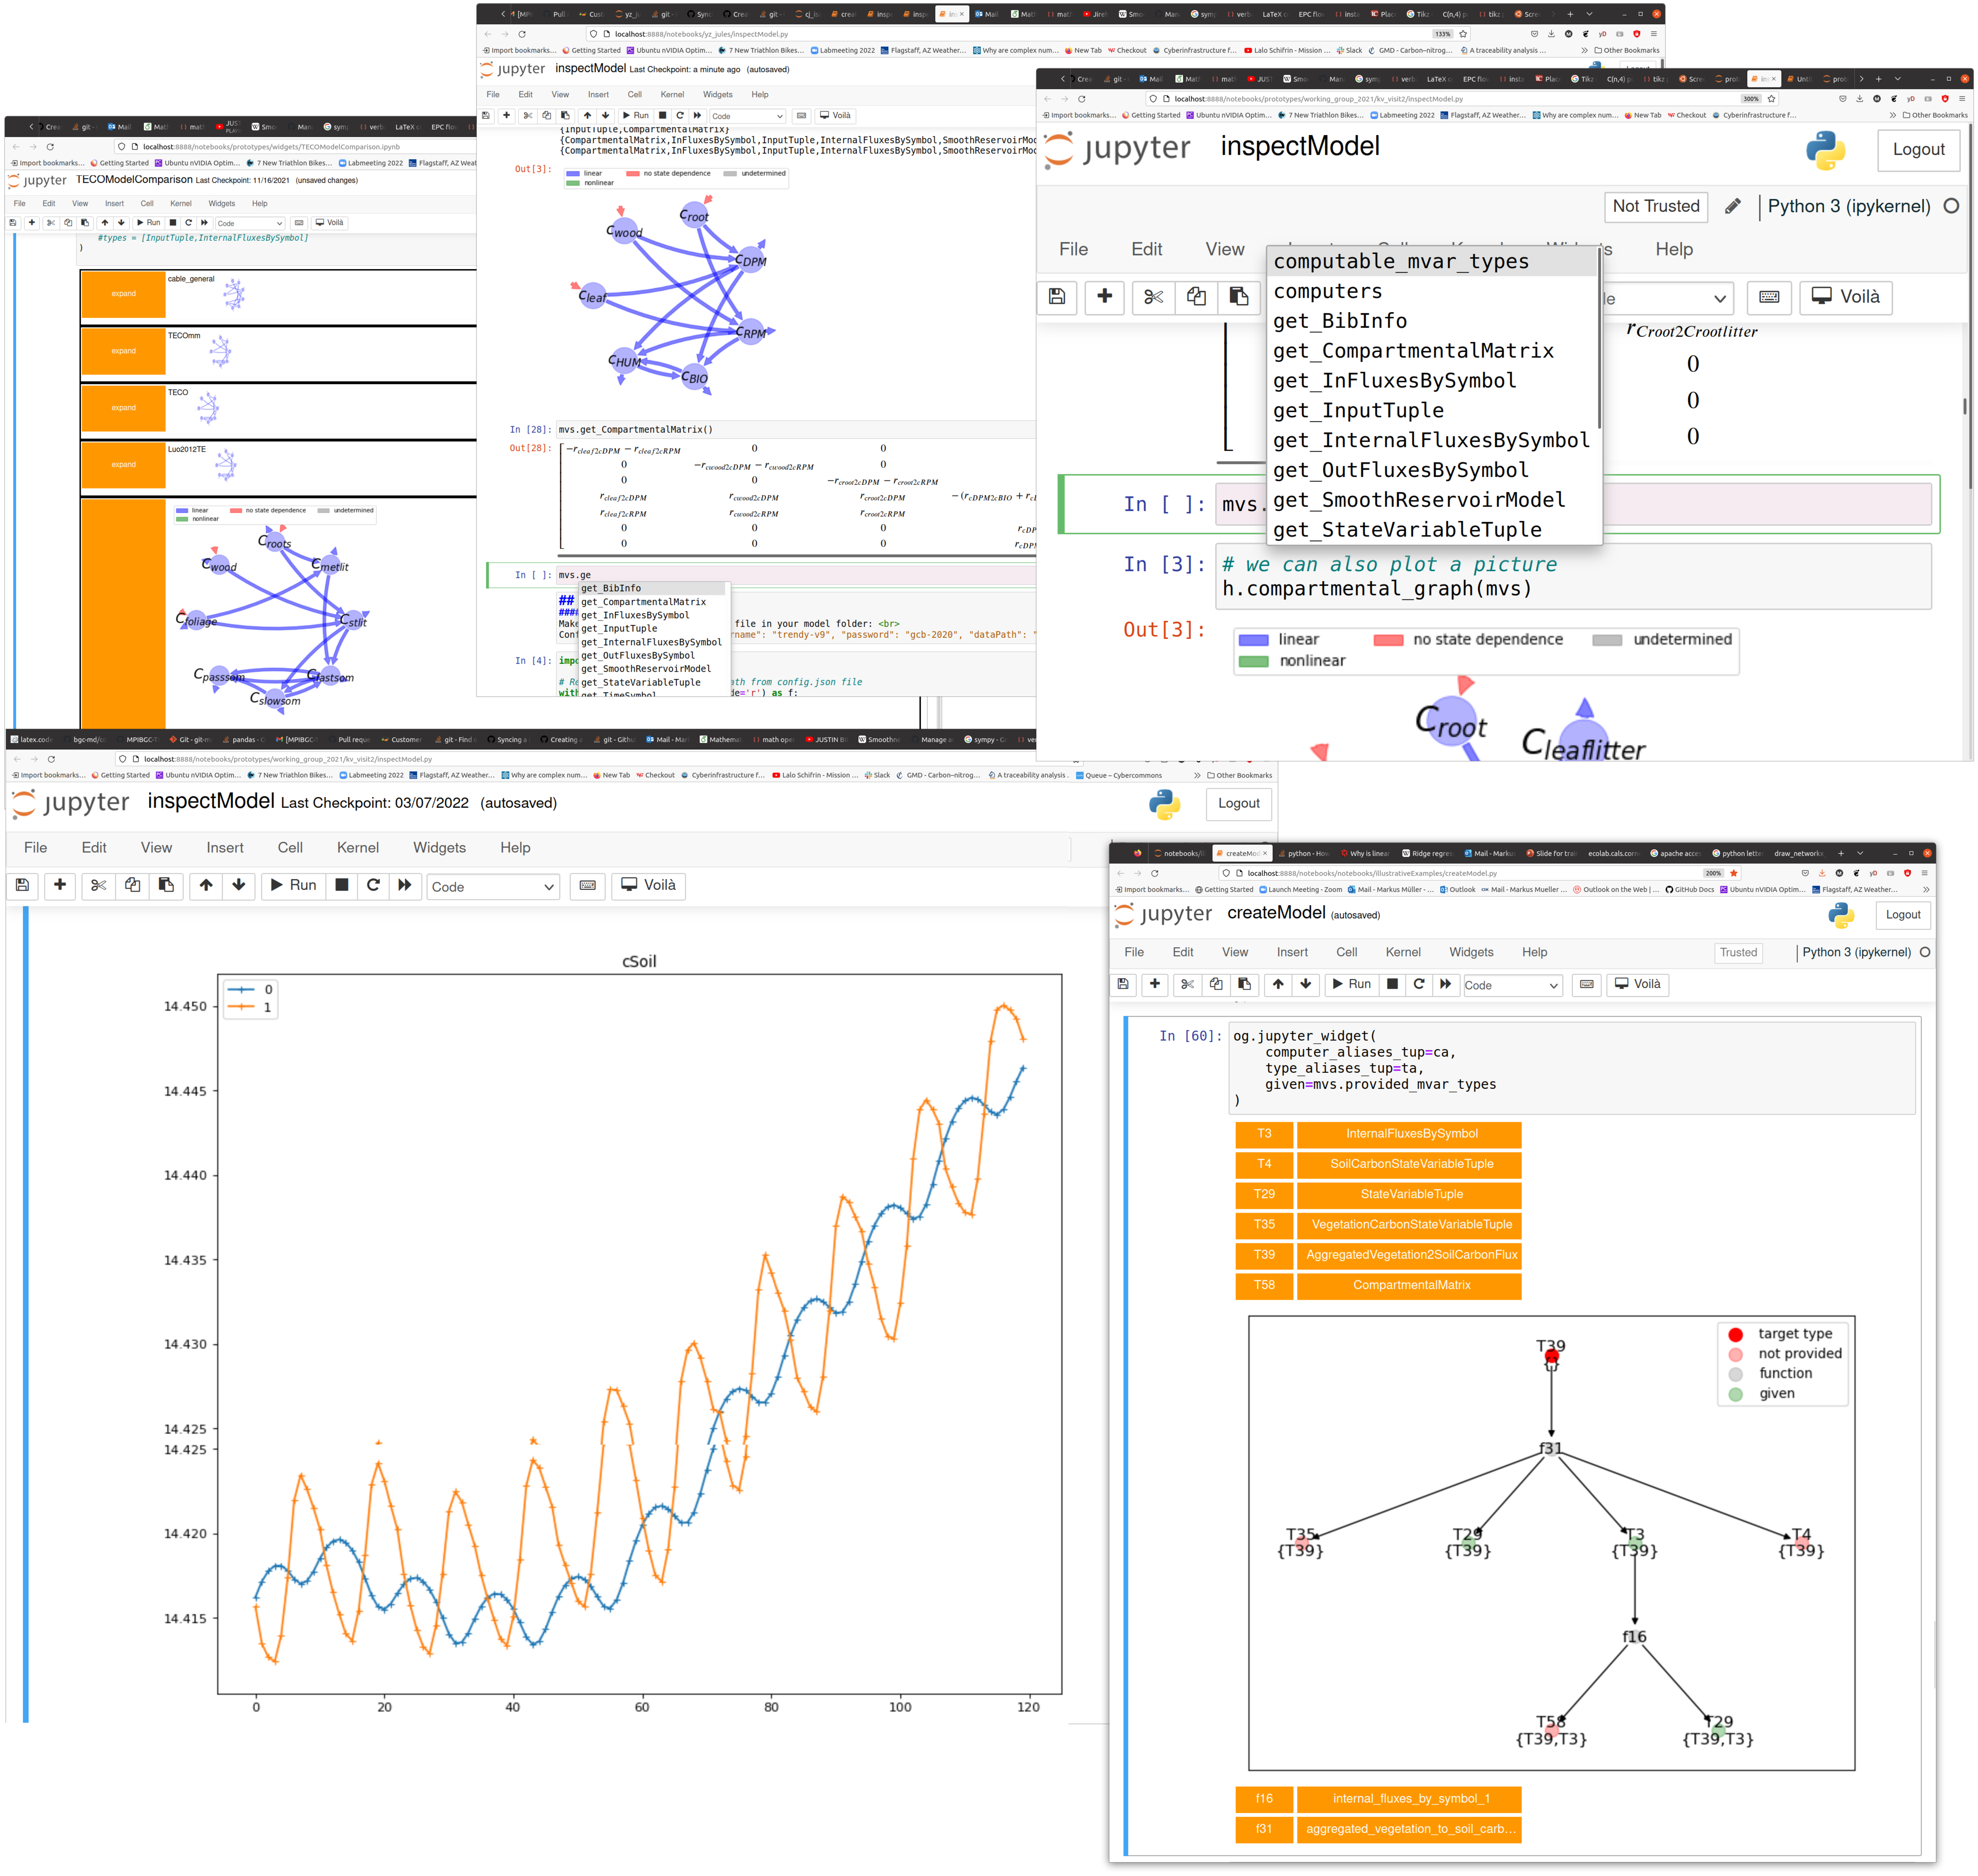
\includegraphics[width=\columnwidth]{TabScreenCombined.pdf}
  \caption{
      Figure description, top row, left to right: Interactive jupiter widget
      with a table of models (orange buttons can be clicked to expand or
      collape a more detailed view of the particular model), Model inspection
      with pool connection graph, which can be derived from the symbolic
      description along other symbolic properties as flux equations and the
      compartmental matrix, Zoom into IPython/Jupyter UI, showing methods
      automatically added by the computability graph library.  \\ Bottom row:
      Data assimilation with an automatically created numeric model (from
      symbolic description), Computability graph for a desired diagnostic
      (aggregated Flux from the vegetation to soil part, showing that the
      additionally needed information to compute the desired result)
  }
\end{figure}

%\subsection{Examples}
As a conceptual proof of the  approach implemented by \texttt{bgc\_md2}
we reconstruct four models of the trendy9 model intercomparison from their description in the literature.
We express them symbolicly, provide some parameters run them with the trendy9 driver data and
compare them with respect to transient mean ages and transit times of carbon
trough the vegetation and soil subsystems.  
While some of the implemented algorithms for compartmental subsystems are novel 
and yet unpublished, this work focuses on the algorithmic and structural proposal for a model collection
i.e. a model data base to facilitate their use for model intercomparison. 
We provide examples based on the global carbon cycle, but the
packages can be used for a large variety of systems in which mass or energy
conservation is required.
The remainder of the article is structured as follows.
In \sectionref{sec:ConceptualFramework} we briefly describe compartmental systems, with some of the details
relegated to \appendixref{appendix:MatrixDerivation}.
We then provide an overview over the main role of the implemented packages in 
\sectionref{sec:PythonPackages}. A brief introduction to example applications is given in \sectionref{sec:ExampleApplications} followed by a discussion of possible present and future use cases in \sectionref{sec:ConclusionsAndOutlook}.




%:
\section{Conceptual framework}
\label{sec:ConceptualFramework}
\subsection{Definition and classification of compartmental systems} 
The most parsimonious and general description of a compartmental system is a graph in
the mathematical sense, which is a tupel of two sets, the set of nodes, and the
set of edges.  In the particular graphs that describe compartmental systems the
compartments (or pools) form the nodes and the fluxes between them and the
exterior the edges.  The fluxes are allowed to be functions of time and the
contents of the pools exclusively. This is usually referred to as `well mixed' or
`kinetically homogeneous' compartments.  

If we assume any arbitrary ordering of the pools we can represent the mass (content of the pools)
by an ordered tuple $\vec{x}$.
Because mass is a non-negative quantity, this vector of mass contents can
only occupy the non-negative orthant of the state-space; i.e. $x \in
\mathbb{R}^n_+$. 
Likewise the mass, that the system receives from outside is represented
by a tuple of mass input fluxes (mass over time) $u \in \mathbb{R}^n_+$.
It has been shown in \citep{Jacquez1993SIAM}
that for smooth enough fluxes, mass is transferred among compartments and released back to the external
environment can be according to rates encoded in a compartmental matrix $B \in
\mathbb{R}^{n \times n}$. 
Therefore, we can write the dynamics of a
compartmental system as a set of ordinary differential equations of the form
\begin{equation} \label{eq:CompartmentalSystem}
\frac{dx}{dt} = \dot{x} = u(x, t) + B(x, t) \, x
\end{equation}
The key property of compartmental systems is, in order for the system to balance mass, that the square matrix $B=(B_{ij})$ exhibits three main properties
\begin{enumerate}
  \item $B_{ii}\leq0\text{ for all }i$,
  \item $B_{ij}\geq0\text{ for all }i\neq j$, and
  \item $\suml_i B_{ij}\leq 0\text{ for all }j$.
\end{enumerate}
Then, $\tens{B}$ is called \emph{compartmental} and governs all internal cycling of material as well as the exit of material from the system.
We describe the relationship between the graph and matrix based descriptions in \appendixref{appendix:MatrixDerivation}.

We distinguish between different types of compartmental systems, according to linearity and autonomy. If the vector of inputs and the compartmental matrix depend on the vector of states in system \eqref{eq:CompartmentalSystem}, we call it non-linear, and linear otherwise. Similarly, if the vector of inputs and the compartmental matrix depend on time, we call the system non-autonomous, and autonomous otherwise. 
Both descriptions of compartmental system, the intuative graph of pools and fluxes and the 
matrix based formulation as an ODE system have advantages for some applications. 
While the graph based description allows for composition of subgraphs and decomposition of models into e.g vegetation and soil part, the ODE descripiton facilitats the description and implementation of some advanced numerical algorithms as explained below.
In our approach both formulations are converted into each other automatically as need arises.
This effortless switching between the viewpoints is the main facilitator of the new level of transparancy of our approach, their combination enables the computation of transit time and mean age systems for subsystems of selected pools with no more effort than defining the pools constituting them.

\subsection{System and sub-system level metrics: contents, fluxes, age, transit time}
Compartmental systems can be described by a set of buildig blocks and metrics. 
We will show later that the formulation of these metrics as return values of
strictly typed functions does make the creation, inspection and
comparison of compartmental systems much more feasable by software tools  
but it can also guide the scientific discussion about what is to be considered a metric.
It is the first of the following criteria:
\begin{enumerate}
  \item
    \label{enum:function}
    In our definition we require that a metric must be unambigiously computable by a function of other metrics or building blocks of a model. 
  \item
    \label{enum:general}
    Preferably metrics should be applicable to all (nonautonomous, nonlinear) compartmental systems, i.e. not rely on e.g. equilibrium conditions.
  \item
    \label{enum:measurable}
  Preferably metrics should also be physical properties
  i.e. have a clearly defined way to measure them at least in principle.
\end{enumerate}

Beside the content of pools the whole system or subsystem and fluxes between
them, ages, and transit times are key quantities of compartmental systems that
fulfill all of these criteria: \enumref{enum:function}, \enumref{enum:general} and
\enumref{enum:measurable}.
They help to better understand underlying system dynamics and to compare models
with different sizes or structures.  They can in principle be measured: While
age describes how old material in the system is, transit time describes how
long material needs to travel through the entire system from entry to exit
\citep{bolin1973Tellus, Sierra2017GCB}.  They are applicable to general
nonautonomous nonlinear systems.  This makes them the first choice for model
comparisons. 

There are metrics that are not suitable to compare \emph{all} compartmental systems because they make further assumptions, e.g. the existence of equilibria. 
General compartmental systems can be nonlinear and nonautonomous, in the latter case making the concept of equilibrium itself meaningless and in the former the computation of the possibly empty set of fixed points by far to difficult to attempt (by a function).
If we wanted to include a strictly typed function to do it, its argument would
have to be of a new type for a linear autonomous system.  Achieving the same flexibility
and complete transparancy w.r.t. flux, rate, or matrix centered description
will necessitate additional types for constant rates or linear fluxes.
We note that metrics build upon equilibrium assumptions fail to meet criteria \enumref{enum:general}.

Another class that fails at least one of the criteria
are properties that can still be unambigiously defined by a function and
therefore computed but are not physical quantities and are therefore to be
considered properties of the model rather than reality. 
\footnote{
  That a flux `rate' should be considered a model property (or latent variable)
  rather than a physical property becomes more apparent when we consider
  processes that treat material of different age or position in the pool
  differently.  In this case the assumption that the material in the pools is
  `well mixed', and can therefore be treated by the \emph{same} exit `rate'
  would be violated, and the model no longer 'compartmental.  However such
  processes clearly exist and fluxes and mass are still measurable.  The
  concept of a single 'rate' applied to all material in a pool is implied by
  the definition of compartmental systems.
} 
Flux rates and compartmental matrices, and more importantly properties derived from them, fall into  this category. 
One example is `turnover time' which is defined as the quotient between between content of and outflux from a pool, or as the inverse of the rate. 
`Turnover time' is an interesting example as it violates, \enumref{enum:measurable} or \enumref{enum:general}, 
because it turns out that for a one pool system in equilibrium it actually coincides with the mean backward transit time
which could be approximated by many measurements but looses this interpretation in any non-equilibrium state.

More recently proposed metrics 
like `carbon storage capacity',  `carbon storage potential' and `residence time' suffer from the same issue.
\todo{
  @Kostia, could you collect the Matrix approach references in the bib file and cite them here?
}
They have a physical meaningful interpretation only in equilibrium 
but loose it if their formal definition is extended to the transient case (nonautonomous compartmental systems) as in \citep{2017}
While we could implement a function applying such a definition, \enumref{enum:function} it would be extremly misleading and violate \enumref{enum:measurable}.
A user asking for  'ResidenceTime' (by applying such a function) would reasonably expect the transient 'time of residence' of material and not the time of residence the material  
\emph{would} have if the system was frozen at this moment \emph{and} allowed to reach its equilibrium.

A simalar restriction of generality applies to applications of Shannon's information entropy as a complexity measure 
of dynamical systems \citep{Ebeling1998}. For nonautonomous linear systems it has 
been used to describe the uncertainty of a particle's path through a
compartmental system, quantifying how difficult it is to predict this path. 
and to compare path properties of models with different number of
compartments and connections among them \citep{Metzler2020}. 
It's use can be extended to systems in equilibrium.

Surprisingly the literature even contains proposals for metrics that can not be defined as functions because they are ambigiously defined like the following matrix factorization approach.  It has been claimed that for most Carbon cycle models the linear verion of \eqref{eq:CompartmentalSystem} can be written in product form.
\begin{eqnarray} 
  \frac{dx}{dt} &=& u(t) + B(t) \, x 
  \label{eq:LinCompartmentalSystem} 
  \\
                &=& u(t) + A \xi K(t) \, x
  \label{eq:AxiK}
\end{eqnarray}
\todo{@Kostia, could you collect the Matrix approach references in the bib file and cite them here?, there is also a reference to a paper of Carlos and me referenced in Yiqi's 2017 paper}
While it is certainly possible to derive \eqref{eq:LinCompartmentalSystem} unambigously from \eqref{eq:AxiK} the opposite direction is not possible. Neither is the form \eqref{eq:AxiK} as general as \eqref{eq:LinCompartmentalSystem} nor is the decomposition uniquely defined.
While the issue with generality could be solved similarly to the equilibrium
issue by introducing subtypes of decomposable matrices and fluxes the issue of
ambiguity prevents the implementation of a function in the mathematical sense, wich requires the return value to be unambigously defined by the arguments.
This actually shows that any analysis built upon the decomposition is not
suited to discuss compartmental systems in general, not even if they can be
written in the form or \eqref{eq:AxiK}. This is relevant since such results have been published without discussion of the inherent ambiguity. We show in detail why this is the case in \appendixref{appendix:MatrixDerivation}.

To summerize, among the traditionally proposed 
metrics for compartmental systems fulfill our conditions of unambigous definition, general applicability to nonautonomous nonlinear and physical interpretability as pricipally measurable. The few that do are:
contents of pools, the fluxes between them and the age and transit times distributions for the whole system or parts of it.  
To provide those metrics for all models is therefore a priorety.

\subsection{Compartmental systems in equilibrium} \label{sec:Equilibrium}
The concept of equilibrium is restricted to autonomous systems. 
It does not even make sense to ask the question otherwise. 
If the autonomous system is nonlinear it is possible but not certain that an
equilibrium exists. The only case where we can expect an equilibrium are
linear, autonomous, pool models, 
\begin{equation} \label{eq:LS}
\dot{x} = u + B \, x, \qquad  \mathrm{with} \quad x(t_0) = x_0.
\end{equation}
for which interesting properties can be
obtained by the \LAPM package.  The equilibrium $x^*$ is defined by the
condition  $\dot{x^*}=0$ which translates to $-B x*=u$ which means that for
pool contents $x*$ the influxes $u$ match the outfluxes $B x*$ exactly.  It is
straightforward to see that for this to happen all 
pools with influxes must be connected (possibly via other pools) to an outflux of
the system, and that the (constant) rates for all the flux rates out of all
pools along this paths are greater than zero, since an input receiving pool $p$
without these conditions would necessarily grow over time, violation the
equilibrium condition $\dot{x*}_p=0$. Interestingly these conditions also
gurantee that $B$ is invertable and the equilibrium therefore uniquely
determined by: 
\begin{equation} 
\label{eq:x_Binv_u}
x^* = - {B^*}^{-1} \, u^*.  
\end{equation}
Although at different times different material moves through the system, the
size of the pools does not depend on time if the system is in
equilibrium: $x(t)=x^*$ 
This is also true for other properties such as the
age distribution of mass in particular compartments and in the entire system
and the transit time distribution, which is defined as the time it takes masses
in the input flux to appear in the output flux. 
Although the material moving through the system does change the amount, age and transit
time distributions do not. 
They are in fact characterized by the Phase Type
distribution, which depends on compartmental matrix $B$ and the equilibrium
solution $x^*$ for the system age distribution and the $B$ and the input $u$
for the transit time distribution \citep{Metzler2018MGS}.
Compartmental systems at equilibrium have similar properties as continuous-time absorbing Markov Chains \citep{Metzler2018MGS}.
Therefore, we can obtain other quantities of interest such as  the path entropy of particles that travel across the system and the occupation time of particles inside compartments \citep{Metzler2020}. These properties of linear autonomous compartmental systems at equilibrium can be obtained with the \LAPM package.

Interestingly the properties of linear autonomous systems in equilibrium can
also be computed for nonlinear systems in equilibrium if such an equilibrium
exists.
\begin{equation} \label{eq:NLS}
\dot{x} = u(x) + B(x) \, x, \qquad  \mathrm{with} \quad x(t_0) = x_0,
\end{equation}
In equilibrium the system is indistinguishable from a linear autonomous one
\begin{align} 
  0= \dot{x^*} = u^* + B^* \, x^*
\end{align}
with $B^*=B(x^*)$ and $u^*=u(x^*)$ 
If the inverse ${B^*}^{-1}$ exists transit time and age distributions can be computed 
\citep{Metzler2018MGS}.
and therefore also  nonlinear autonomous
systems at equilbrium can be analyzed with the by the
\LAPM package.
Note however,that 
\eqref{eq:x_Binv_u} is useless to determine $x^*$ and 
no such $x^*$ might exist for some systems
while others may have multiple fixed points and the age and
transittime distribution may be very different for these different equilibria.

%%%%%%%%%%%%%%%%%%%%%%%%%%%%%%%%%%%%%%%%%%%%%%%%%%%%%%%%%%%%%%%%%%%%%%%%%%%%
\subsection{Time evolution} \label{sec:trajectory}
We consider now linear non-autonomous systems of the form
\begin{equation} \label{eq:NALS}
\dot{x}(t) = u(t) + B(t) \, x, \qquad  \mathrm{with} \quad x(t_0) = x_0.
\end{equation}
In this case, the inputs and the compartmental matrix are time-dependent and
the system never converges to a fixed-point solution. In most cases, an
analytical solution cannot be obtained, but the solution can be 
obtained numerically. In particular, the solution for systems of the form of equation \eqref{eq:NALS} can be written as
\begin{equation}
x(t, t_0, x_0) = \Phi(t, t_0) x_0 + \int_{t_0}^{t} \Phi(t, \tau) u(\tau) \mathrm{d}\tau.
\end{equation}
The state transition operator $\Phi(t,t_0)$ is a matrix-valued function that
multiplied with the state $x_0$ at $t_0$ transitions it to the state $x(t)$
subsequent time $t > t_0$. It is numerically computable by solving an matrix
ode derived from \eqref{sec:trajectory} 
From $\Phi(t,t_0)$ we can obtain not only the temporal evolution of the
solution $x(t)$ but also of the distributions of ages of the mass in the compartments and in the entire system \citep{Metzler2018PNAS}.
The \CompartmentalSystems package provides all the functionality necessary to do these computations, which rely on a description of the time-dependent input vector $u(t)$ and the compartmental matrix $B(t)$, as well as initial age distributions for the compartments.

Furthermore, these computations can also be obtained for nonlinear systems of the form
\begin{equation} \label{eq:NANLS}
\dot{x}(t) = u(t, x) + B(t, x) \, x(t), \qquad  \mathrm{with} \quad x(t_0) = x_0.
\end{equation}
by numerically solving \eqref{eq:NANLS} and plugging the solution $x(t, t_0,
x_0)$ back into it, which results in $\tilde{B}(t)=B(t,x(t, t_0,x_0))$ and
$\tilde{u}(t)=u(t,x(t, t_0,x_0)$  i.e a linear system in the form
\eqref{eq:NALS}. 
Therefore,  age and transit time
distributions can be obtained for nonlinear non-autonomous systems along the
specific trajectory. Detailed methods for the computation are provided in
\citet{Metzler2018PNAS}

%\section{Software description}
\section{The \python packages}
\label{sec:PythonPackages}
\subsection{\LAPM}
Linear Autonomous Pool Models (\LAPM) is a python 3 package for the study of autonomous compartmental systems at equilibrium such as those described in section \ref{sec:Equilibrium}. 
It implements the LinearAutonomousPoolModel class, with methods for the
symbolic and numerical solutions of the steady state content in the compartments, and the steady state release out of the compartments. For transit time, system age, and pool age, it provides symbolic and numerical computations of distribution densities, cumulative distribution functions, mean, standard deviation,           variance, higher order moments, and Laplace transforms. 

For the analysis of compartmental systems in analogy to absorbing Markov chains, \LAPM provides methods for the computation of the entropy rate per jump, the entropy rate per unit time, and path entropy. It provides the class DTMC (discrete-time Markov chains), with methods to compute the fundamental matrix, stationary distribution, and expected number of jumps of the Markov chain.

\subsection{\CompartmentalSystems}
This package deals with non-equilibrium trajectories of compartmental systems.
In particular, it provides the class smooth\_reservoir\_model to describe
symbolically the general class of non-autonomous nonlinear compartmental
dynamical systems of equation \eqref{eq:CompartmentalSystem}. It does not
require code for numerical computations or model simulations, but rather defines the underlying structure of the respective model. 
All fluxes or matrix entries are expected to be SymPy expressions. 

To obtain numerical results, the package
provides the class smooth\_model\_run, which is initialized with the initial
conditions of the system of equations, a set of parameter values, and a time
sequence. It computes the solution trajectory for the given initial conditions and
parameter values , finds the corresponding linear system with the same solution
following the strategy described in section \ref{sec:trajectory} computes the
state transition operator $\Phi(t, t_0)$ for these solution trajectoriess and 
provides methods to obtain time dependent densities with corresponding moments and quantiles for system age, compartment age, and transit time. 

An additional module provides functions to obtain initial age distributions
required for the computation of time-dependent age distributions. 
This module uses \LAPM.

\subsection{\ComputabilityGraphs}
This package was specifically developed for use in \texttt{bgc\_md2} but is also usable in separation.
It allows a declarative description of results (model properties) i.e. completely abstracting from the way they are obtained as e.g in a \texttt{Make} 
%\citep{
%Feldman, S. I. (April 1979). "Make --- A Program for Maintaining Computer Programs". Software: Practice and Experience. 9 (4): 255–265. CiteSeerX 10.1.1.39.7058. doi:10.1002/spe.4380090402. S2CID 33059412
%} 
\footnote{Which won the ACM software system award in 2002} file.  This
abstraction is the precondition for queries as in other declarative languages
like e.g. \texttt{SQL}, whose purpose is the comparison of data, as opposed to
the implementation of data base software.  Comparison of models w.r.t. their
predictions poses a similar challenge: The amount of e.g. Carbon or Nitrogen in
a compartmental system or their ages or transit times through it are (in
principle) measurable quantities. They do not change if the description of the
model is changed from a graph (pools and fluxes) to a matrix or a product of matrices.
Instead of forcing a user of the data base to use a fixed
description it is much more desirable to allow as many equivalent ones as
possible \emph{and} make the equivalence explicit by  well defined mappings i.e. \emph{functions}.

\ComputabilityGraphs facilitates exactly this.
It implements a class \texttt{CMTVS} which stands for 
{\bf C}onnected {\bf M} ulti {\bf T}yped {\bf V}ariable {\bf S}et. 
Instances consist of a set of variables with unique type (only one variable per type) and a set of type annotated functions that exclusively 
use these types in their signature (as arguments or return values) which we call \emph{computers} from now on.
This combination implicitly implements a declarative model description language to describe results of computations by requesting the type of the result. 

It also confines what we consider a model property, building block or
metric. The network of functions using these types as arguments or return values
enforces an unambigous defintion, which prevents the description of models to
become vague, e.g. the compartmental matrix is a function of the internal and outgoing fluxes and the ordering of the state variables.  
This rigorous description actually defines computability graphs that we exploit mainly in the followng ways.
\begin{enumerate}
  \item
  \label{enum:computable}
  To compute which types of information (target results) are obtainable given the types of the provided variables. 
  Since a \texttt{CMTVS} instance knows the types of all its variables and the signatures of all
  available functions, it can iteratively add the result types of all applicable functions until no
  more result types can be reached. This is a forward graph search.
    \begin{figure}[h]
      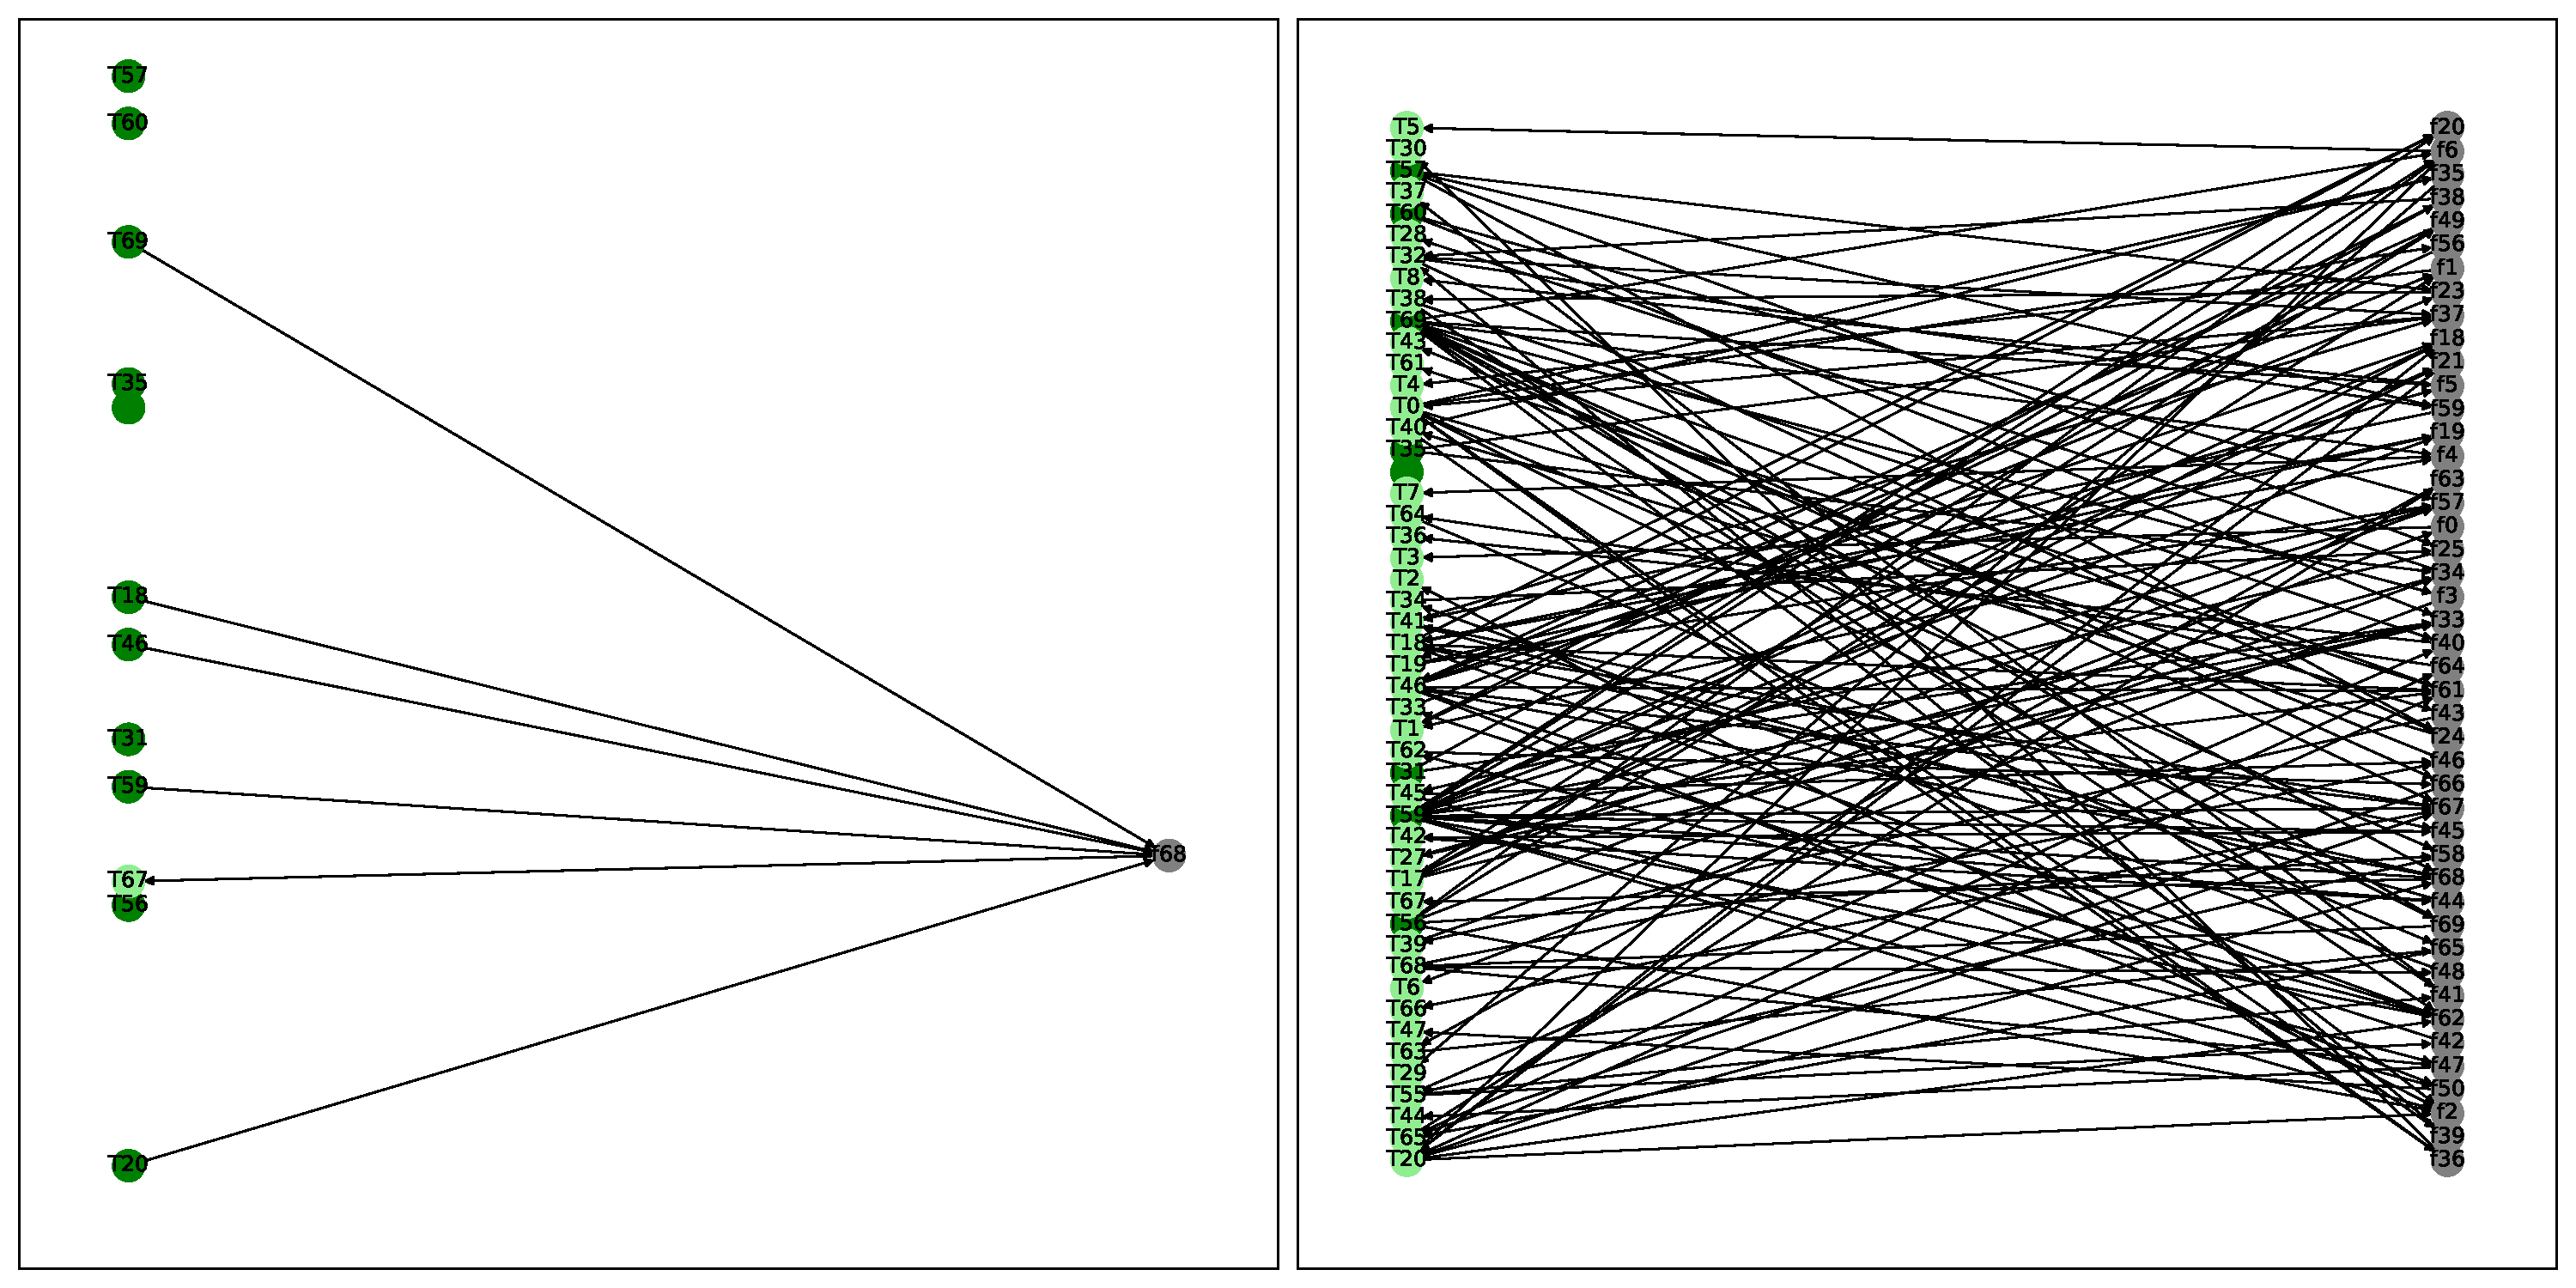
\includegraphics[width=\textwidth]{closure.pdf}
      \caption{Closure under computability} 
      The left hand side picture shows a first step in the computation of the
      computable types.  We find a first applicable (i.e. all its arguments are
      given) function (grey node on the right), infer the result type from its
      type annotation and add it to the set of given types (new light green
      node).  Now we have more arguments and thus more possibly applicable
      functions.

      The right hand side plot shows the result of the recursive application of this
      procedure to a \texttt{CMTVS} instance (in this case describing the YIBS model).
      Without performing any actual computation we know which results we can
      compute (30 light green nodes) from the 11 provided variables (dark
      green), some of them in different ways via intermediate results
      (as explained in  \figref{fig:dep_graph} below) .  This
      information is used to automatically add methods to an \texttt{CMTVS}
      instance, so that interactive python environments suggest computable
      results to the user. In this case 30 new methods appear automatically, including very complex results like the pool specific transient 
      mean age solution for the vegetation carbon sub system witch appears as \texttt{get_NumericVegetationCarbonMeanAgeSolutionArray()}
      It is also the basis for queries, e.g. "for which
      models can we compute the mean transit time through the 
      the vegetation subsystem?"  Note that the applicable functions (in this
      example 45 represented by the grey nodes) can also be used
      independently of the \texttt{CMTVS} class, explicitly by the user. 
      A lack of the automatic combination would however make it much more difficult to
      guide a user through the often purely technical conversions to the
      targeted result and massively increase the amount of necessary
      handwritten documentation.  In this sense \ComputabilityGraphs can be
      used as computable documentation or a much simpler API.  
    \end{figure}
  \item
  \label{enum:deptree}
  To find out what type of information is 
  \emph{missing} to obtain a 
    target variable (backward search).  
  \figref{fig:dep_graph} shows the bipartite dependency tree for a quite complex numerical result.
  printed by the \texttt{CMTVS} instance. 
  The red node T35
  at the bottom represents the target that we want to
  compute: \texttt{NumericVegetationCarbonMeanBackwardTransitTimeSolution}
  The green nodes are the building blocks that we have provided in the
  model source file.
  The light red nodes show things that are not provided but have to be 
  computed via the function represented by the grey nodes. 
  This is possible if all their (ultimate recursive) dependencies
  are green nodes. 
  In this example this is the case except for nodes  T70 and T38
  \item
  \label{enum:compute}
  To compute the actual result of a targeted type.
  If a result type is in the computable set determined by \ref{enum:computable} then 
  The search tree created under \ref{enum:deptree} can be traversed in reverse starting
  at the given nodes and ending in the final result.
  \texttt{StartConditionMaker} and \texttt{VegetationCarbonStateVariableTuple} respectively 
\begin{figure}[h]
  \label{fig:dep_graph}
  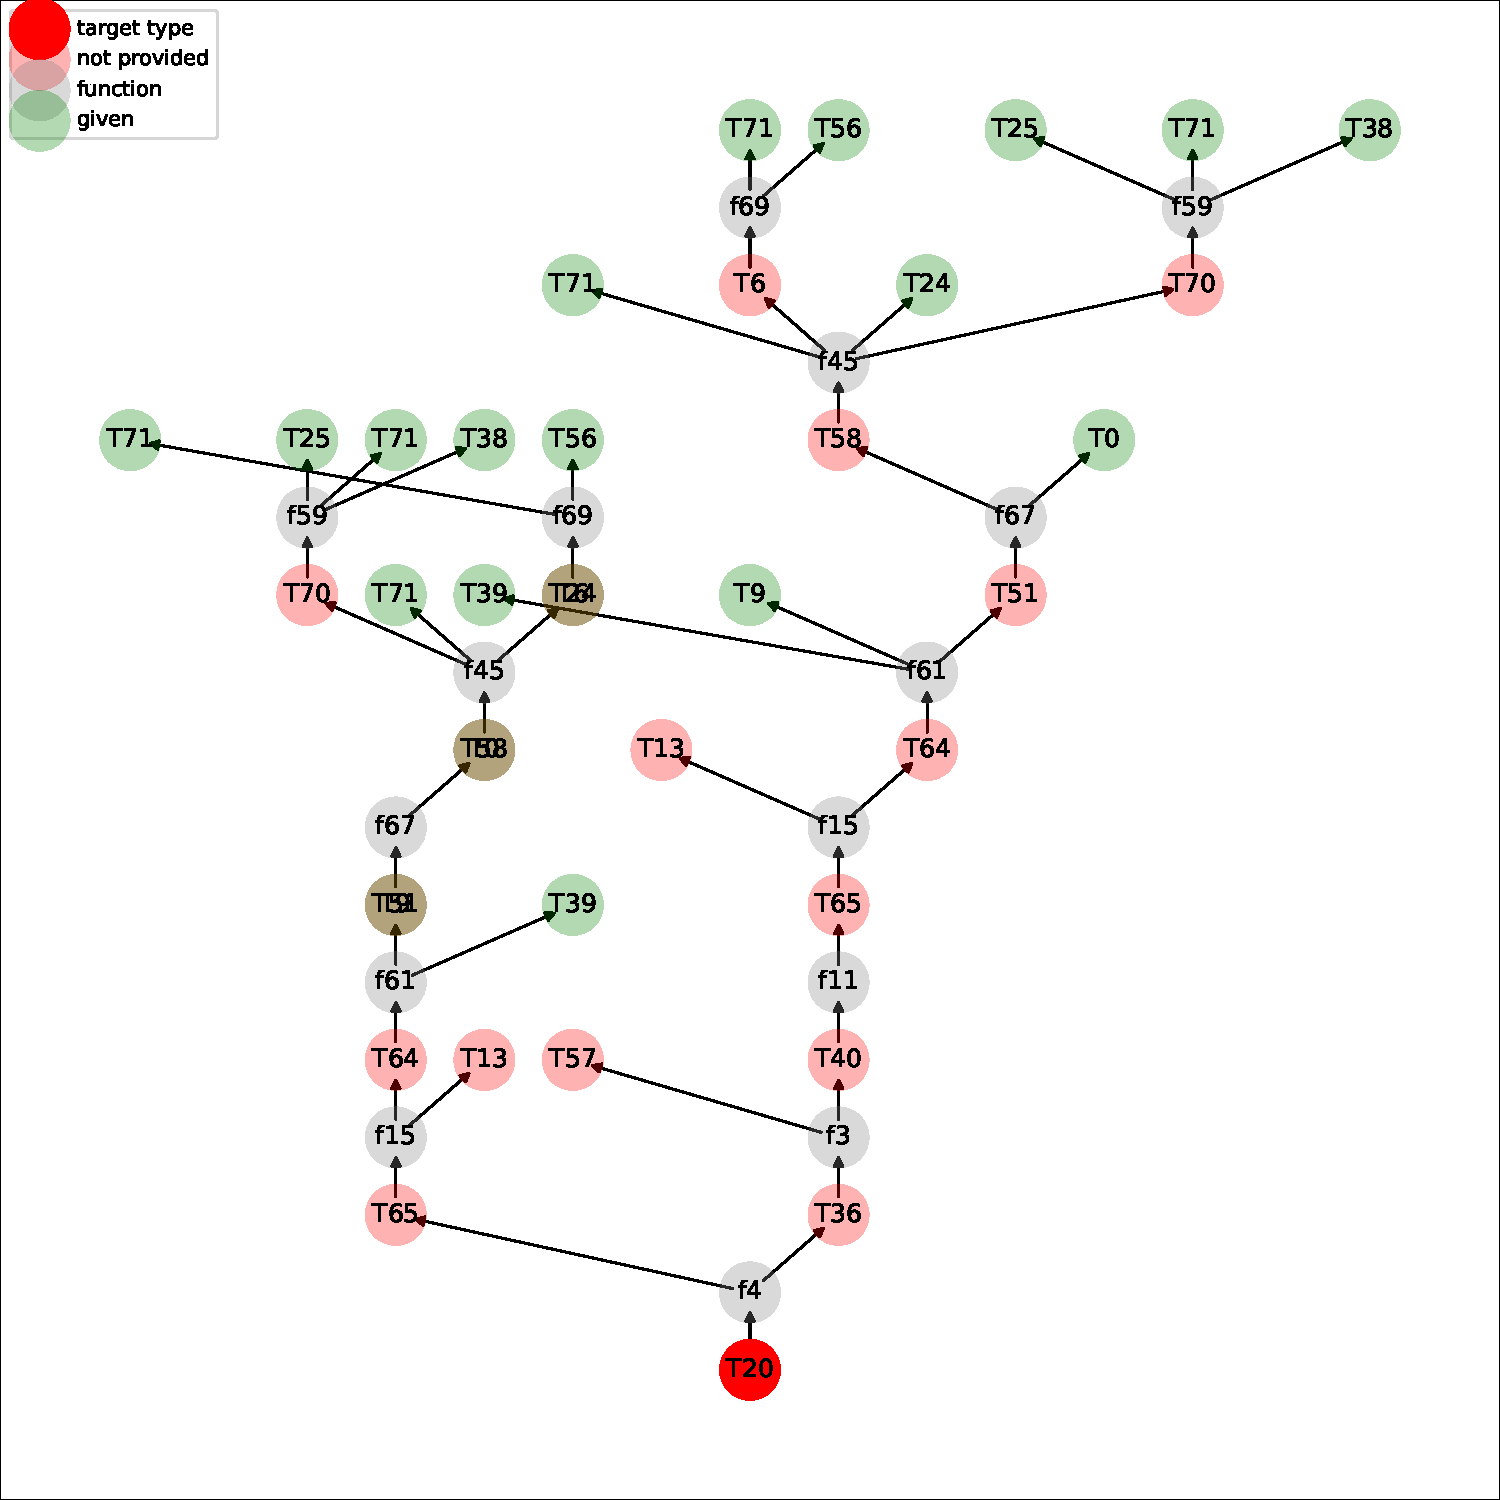
\includegraphics[width=\textwidth]{dep_graph.pdf}
  \caption{ Dependency graph}
  {
    \small
    JAMES/TypeLegend.tex
  }  
\end{figure}  
\end{enumerate} 
Using \ref{enum:computable} and \ref{enum:compute} together a
\texttt{CMTVS} can add get methods for computable results dynamically.  This
is very useful for for the user interface in interactive python sessions,
including jupyter notebooks since on pressing the tab key, the python
interpreter suggest available method calls as autocompletion options for any
object followed by a "." For an \texttt{CMTVS} object these methods become
more numerous automatically as more and more information is added to it.
Apart from the user interface \ref{enum:computable} is necessary for queries.
If we have a (large) set of different \texttt{CMTVS} objects and want to
compare them with respect to a certain property, we must first find out for
which of them this property is actually computable.  A welcome side effect
of the \text{CMTVS} model description language is the possibility to include
models about which we know very little. In a traditional database these
record would most likely be incomplete, whereas here we just get offered
fewer computable results.  
This is especially useful for the creation of new
models, in the process of which one naturally starts with a small set of
variables that is gradually extended.
Typically one of the first steps is a dictionary of symbolic flux equations, which already allows the visualization
of the compartmental graph or flow diagram , symbolic matrices and vectors and is extremly useful for debugging.



\subsection{The biogeochemical model database \texttt{bgc\_md2}} This is the
central package and can be seen as a frontend to \CompartmentalSystems and
\LAPM facilitated by \ComputabilityGraphs.  For the following discussion it is
important to note that \texttt{bgc\_md2} is a library, rather than a framework,
since there is no `inversion of control', i.e. \texttt{bgc\_md2} as well as all
the other packages are called from normal python code, rather than
\texttt{bgc\_md2} calling user code in a restricted execution environment as a
framework would do.  Although internally \ComputabilityGraphs acts like an
extended  compiler  (not only testing type consitency of function calls but
actually suggesting them) for a DSL taylored to the domain of compartmental
models, it is technically represented by \texttt{bgc\_md2}'s API (consisting of
the provided datatypes, functions, and the dynamically created methods of the
\texttt{CMTVS} objects for computable properties).  This makes it much more
flexible to use than a framework. We can use the full toolset of the
\emph{python} ecosystem to create instances of the model building blocks and to
postprocess results afterwards.  While any comparison requires standards i.e.
rigorously defined properties which can be formulated for all models and
therefore naturally surpresses idiosyncracies of models, it can be very helpful
to use these idiosyncracies for the creation of a model.  This is possible
since we can use absolutely unrestricted python code to create the model
building blocks.  Imagine for example a model that includes pools in many soil
layers with similar conecting fluxes. A model description code using
\texttt{bgc\_md2} could use loops to express this.  This also applies to
postprocessing. Some of the functionality in \LAPM and \CompartmentalSystems is
not generally applicable to \emph{all} models in \texttt{bgc\_md2}'s collection
and therefore cannot be offered by the `computers'. There is however no reason
to prevent a user to apply them (or any other bit of code) to the results of a
\texttt{bgc\_md2} computations.  Armed with this flexibility we know that our
DSL does not have to provide everything and can restrict it to sensible categories
for comparisons.
%\subsubsection{Provided Types and Computers}
\texttt{bgc\_md2} provides:
  \begin{enumerate}
    \item
      Datatypes defining {\bf building blocks and comparable diagnostic results} 
      specifically tailored to compartmental models, 
      e.g.\ \texttt{CompartmentalMatrix}, \texttt{InternalFluxesBySymbol},
      \texttt{NumericVegetationCarbonMeanBackwardTransitTimeSolution} \dots  
      specifically including the symbolic expressions for pool contents, in- out- and internal-fluxes for
      subsystems, single pools or the entire model, as well as their numerical counterparts obtained from 
      by solving the parameterized IVPs and the most general diagnostics e.g. transient mean-age and transit time solutions.
      Since many these types are based on a symbolic
      mathematical representation, using \sympy, many symbolic results are computable 
      without the need to know parameters or data to run the models.
      Using the underlying graph representation as sets of pools and fluxes, we can reorder pools and thereby automatically transform the compartmental matrices, group them into different subsets (e.g. vegetation, soil, litter, carbon, nitrogen \dots ), substitute pool names, get mathematical expression for cumulative fluxes e.g. from vegetation to soil or simply plot the graphs.
      Using this symbolic transformations we can compare models that might have looked very different initially, simply due to arbitrary choices of pool names or their even more arbitrary order in which they appear. 
      \todo{green brown graph or link to the compare TICO notebook }
    \item
      A set of type annotated functions (from now on called computers) operating on those types,  which combined
      by \ComputabilityGraphs facilities form a much simplified 
      interface to \emph{many  algorithms} in \texttt{CompartmentalSystems} and \LAPM to compute diagnostic variables
      for \emph{many models} in \texttt{bgc\_md2}.
      A complete list can be produced by a single command
  and is added to \appendixref{appendix:listing}
      A very simple example is depicted in \figref{fig:subsystems}.
      \begin{figure}[h]
      \includegraphics[width=\textwidth]{"kv_visit2_veg_soil_decomposition.pdf}
      \label{fig:subsystems}
      \caption{Automatic decomposition into subsytsems} 
      Assuming that a compartmental system has been defined symbolically e.g. by providing expressions for input,  output and internal fluxes different flow diagrams can be created automatically. 
      The additional information for the decomposition into subsystems just consists of a set of pool names for each subsystem.
      (Here vegetation and soil part for the visit model reconstruction).
      For special subsystems like vegetation or soil that frequently occour in Carbon cycle models a declaration of a set of e.g. soil pools has far reaching consequences. 
        Apart from the graph shown here, such a statement immediately makes several new diagnostics available, including matrix descriptions for the vegetations subsystem as in \citep{VeronikasTheoreticalBiologyPaper} or their soil equivalent, cumulative fluxes between the two subsystems as well as transient age and transit time distributions w.r.t. the vegetation or soil subsystems.
        
      \end{figure}
    \item
    $30+$ vegetation, soil or ecosystem models for carbon and nitrogen cycling
      as reusable python modules using the building blocks in a flexible way. 
  \end{enumerate}

\subsubsection{Intentionally Missing Computers}
It is also interesting to note what \texttt{bgc\_md2} intentionally does not implement:
A trivial example is that the computation of equilibria is missing from \texttt{bgc\_md2}'s set of strictly typed functions. 
While we can easily compute the uniqly defined fixed point of a linear
autonomous system, and indeed provide functions to do so in \LAPM, we have to
resist the tempation to make them available via \texttt{bgc\_md2}'s set of
types and computers for \emph{all} compartmental systems. 
This restriction also pertains to equilibrium start age distributions. 
If they simulation is to be started from an equilibrium this is reflected not only by the correct equilibrium
but also a specific age distribution.  
At the moment neither equilibria nor the start age distributions 
are inferred automatically, but have to be provided per model by 
user code to clearly define responsibilities (although, thanks to \LAPM, the usercode amounts ot only three lines).
While we could in the future provide special types for liner matrices or
fluxes, constant rates, along with their appropriate constructors implementing
automatically testable criteria for accidental misdeclaration, implement
computers for them and thus formalize comparisons between linear models
this has not been done yet and such results are not suggested automatically by \texttt{bgc\_md2}.
Users can however use the many functions in \LAPM or \CompartmentalSystems directly.

We also avoid `computers' depending directly or indirectly on ambigiously defined matrix factorizations, 
as we mentioned above and in explained in detail in \appendixref{appendix:MatrixDerivation}. 
These computations can still be performed aided by  \LAPM or \CompartmentalSystems on intermediate results
provides by \texttt{bgc\_md2} computers but also not automatically, since results would be ambigious (in contradiction to the mathematical definition of a function which is our criteria  for admission). 


%%%%%%%%%%%%%%%%%%%%%%%%%%%%%%%%%%%%%%%%%%%%%%%%%%%%%%%%%%%%%%%%%%%%%%
\section{Example applications}  
It is impossible to fully exhibit the potential of this approach without
examples.
To this end we created some illustrative \texttt{jupyter} notebooks that are
availble via binder online without the need to install the packages. 
This paragraph contains only pointers to those much more elaborate notebooks
and some example plots from them.
The examples demonstrate how \texttt{bgc_md2}:
\begin{enumerate}
\item 
  Symplifies and unifies the creation of a new model from scratch while using the
  symbolic and graphic diagnostic capabilities to inspect it while we build it
  and use 
  \ComputabilityGraphs to point out what missing information we have to
  provide to make desired results computable.
  This is demonstrated in
  %\url{}
\item 
  How a model that is already part of the database can be
  inspected w.r.t complex diagnostics like the transient mean transit time that
  would take years to implement in stand alone model code but are now available
  for all models with sufficient information.
  This is demonstrated in
  %\url{}
\item 
  aided by \ComputabilityGraphs 's ability to compute which properties are computable
  allows to query the collection of models that are already part of
  \texttt{bgc\_md2}.
  This is demonstrated in
  %\url{}
\item 
  Several Models for which numeric parameter values and driver data are
  available can be compared w.r.t. abstract properties.
  We chose the mean age and transit time of the vegetation and soil subsystems
  since they are defined for all models while the concrete pools of the models
  differ and not only have different names but also different meaning.
  %\url{}
\end{enumerate}

\begin{figure}[t]
	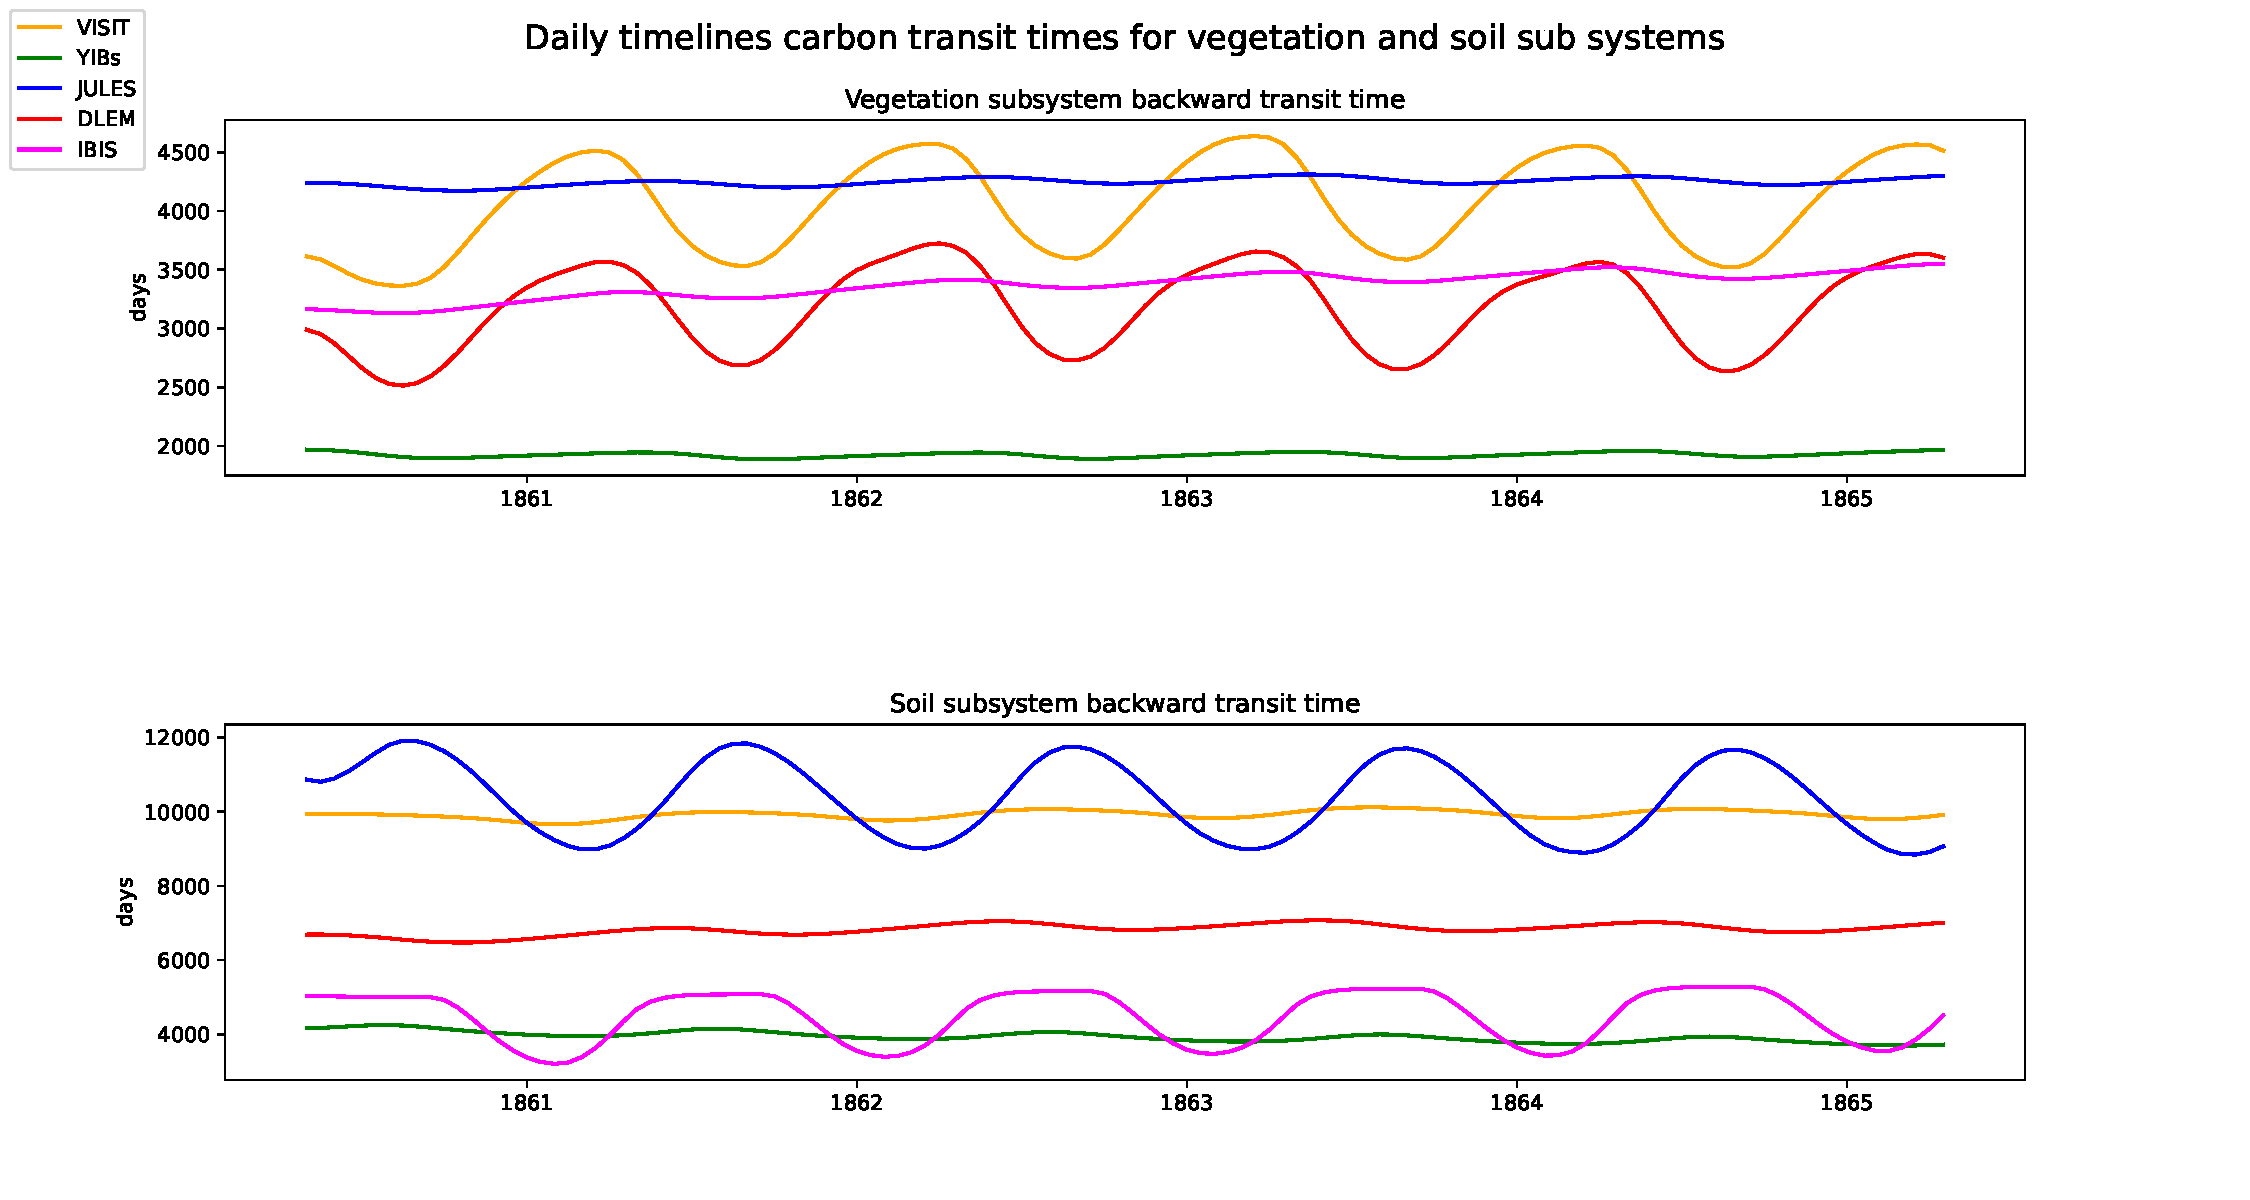
\includegraphics[width=\columnwidth]{test_veg_soil.pdf}
  \caption{
  Figure above: Comparing the (real = transient) backward transit time through 
  subsystems, accross different models. 
  }
\end{figure}  

\begin{figure}[t]
	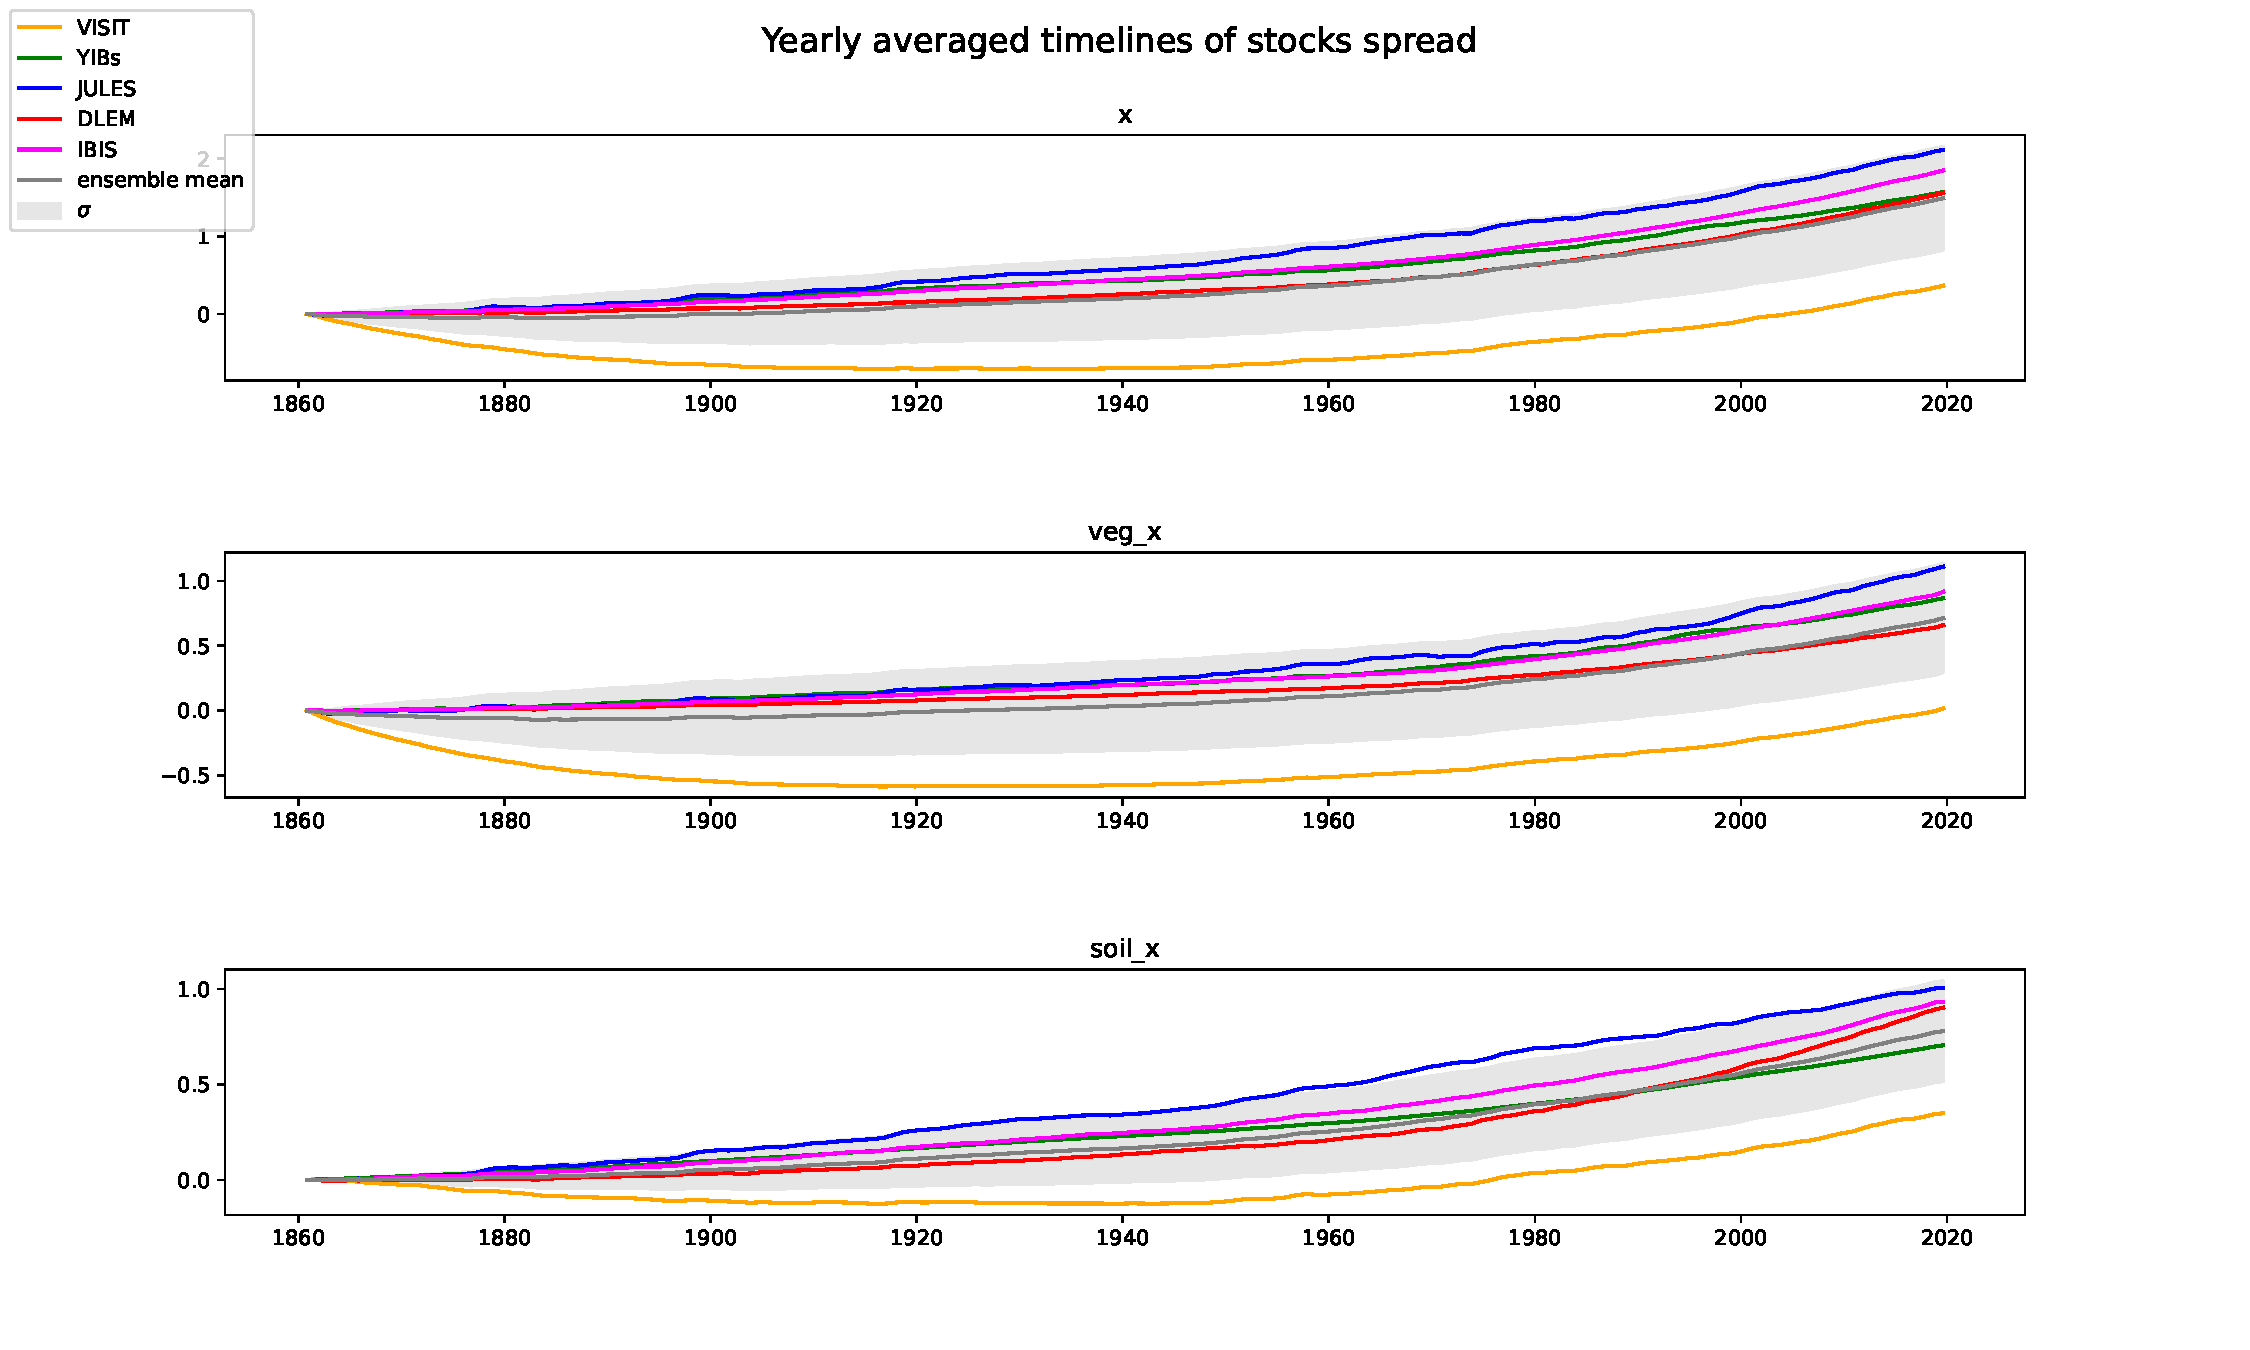
\includegraphics[width=\columnwidth]{test_stock_mean.pdf}
  \caption{
  Figure above: Total Carbon stock and subsystem stock development for different models.
  \texttt{bgc\_md2} only needs to be told which pools belong to which subsystem.
  }
\end{figure}  


\section{Conclusions}
We presented a practially implemented tool for the creation, collection, inspection and comparison of compartmental models and demonstrated how it could be applied 
quickly to the practical problem, of comparing several models with respect to a numerical result complex enough to make its implementation on a per model basis prohibitively expensive,but measuarable in practice.
We created examples to teach new user how use the existing capabilities, how to 
query the collection and how to add models to it.
These immediate practical benefits are suffient for many simple application and are to our knowledge unprecedented. 
In the process some lessons have been learned, that could be very valuable to anybody undertaking a similar project or interested in extending our work.
\subsection{Maintenance}
Creating collections of many models and many metrics 
consistently applicable to all of them is hard,
finding well defined ways to allow users to 
contribute even harder, documenting them comprehensively 
harder still.
The necessity for rigorous definition, absolute clarity and avoidance of 
duplication becomes more and more important as the colletion of models grows.
While we have reached a point where the contribution of new models is easy enough 
to be done by the users of the software, implementation of new features will likely
require the permanent attention of a technical project lead for 
the lifetime of the project, since occasional refactoring is likely to be necessary
to keep the codebase maintainable.
\subsection{Possible Extensions and Iprovements}
\subsubsection{Documentation}
Our software tools are written in \python. 
This has advantages:
\begin{itemize}
  \item
  The availability of hundreds of libraries for pre or postprocessing of model building blocks or results.
  \item
  The flexibility of a very permissive dynamically typed language which allows for rapid prototyping and interactive use of the tools we created.
\end{itemize}
but also disadvantages: The same permissiveness that allows for rapid prototyping and interactive use can also make the detection of unitended misuse harder.
In strictly typed languages like Haskell many unitended usecases are already detected at compile time and reported as errors.
This 'fail early and hard' philosophy ,facilitates the creation of 'fool proof'
'software', whereas interactive environments, notably  R and python follow
almost the opposite approach.  They try their best to make sense of anything
thrown at them which can delay the detection of an error and theirby remove the effects from the cause.
Complex libraries like \texttt{bgc\_md2} which sits on top of \CompartmentalSystems which sits on top of \LAPM which sits on top of \texttt{numpy}, \texttt{SciPy} and \texttt{SyPY} 
needextra care to filter out user input that could cause trouble further down the call stack. This becomes more important the less obvious the computation in question is. 
While an example makes the user aware of her responsibility for correct adaptation, the same user will expect the API of a `black box' to be 'fool proof'. 
This is an ongoing task: While \LAPM and \CompartmentalSystems are pretty well documented 
\todo{Big Thanks to Holger!!!} 
\texttt{bgc\_md} and \ComputabilityGraphs are not yet and none of the packages is `fool proof'. 


\subsubsection{Algebraic Types}
The sets of `computers' and their argument and result types is by no means comprehensive.
In fact there are many results that could be implemented quite easily. 
E.g. we implemented the two types \texttt{VegetationCarbonStateVariableTuple} and 
\texttt{SoilCarbonStateVariableTuple}. It would have been easy to created something similar for e.g. Nitrogen. However the number of types would quickly become large since their
are also related types that would have to be duplicated, i.e. \texttt{NumericVegetationCarbonSolutionArray} or \texttt{NumericVegetationCarbonMeanBackwardTransitTimeSolution} ...
It would be more elegant to express these relationships between types by a concept called
algebraic data types which is used e.g. in  Haskell but also available in \python 's type hint syntax but not yet implemented in \ComputabilityGraphs.
The concept is actually very simple as e.g. a type that uses another type as parameter like alist of integers \texttt{List[int]}. Algebraic types would give us a bigger namespace for less awkward type names and also avoid some boilerplate code for the `computers'.
Another related extension of \ComputabilityGraphs is to allow `computers' that return tuples . 
This could be used to minimize the number of recursive computer application for sets of desired results.   

\subsubsection{Automatic Code Generation and Integration into Earth System Models}
\texttt{bgc\_md2} uses symbolic math to describe the model equations. It then
uses \sympy's facilities to first translate these expressions into regular python code and execute it in a special environment that can be influenced.
\sympy provides a printer module that allows the translation of \sympy expressions to many different programming languages including but not limited to C, Fortran, Java, R and Julia.
So that models could also be translated to these languages automatically. 
A possible application of this ability would be to automatically compile different landcarbon models from \texttt{bgc\_md2}'s collection into an earth system model without the need to reimplement them in the targeted language. 



%\subsection{Installation, documentation and demonstrations}
%The four packages are managed under version control in GitHub, and are publicly available for their evaluation, use, and further modification. 
%
%The four packages can be installed following the instructions provided for the
%installation of \texttt{bgc\_md2}, which depends on \LAPM and
%\CompartmentalSystems and \ComputabilityGraphs. 
%Several installation scripts exist that installs all packages at once. 
%the standard one using Conda. 
%All packages have extensive testsuites which are triggered by every commit but
%can also be run manually e.g. after installation which we strongly recommend.
%The test suites are  stored in the folder \texttt{tests} under the root of the repo . If they run successfully, then all the functionality of the four packages is readily accesible. 
%
%Detailed instructions of the installation procedure can be found in the `README.md' file of the \texttt{bgc\_md2} repository. 
%
%We use standard python docstrings to document modules, functions, classes and methods which are
%available in interactive python sessions. 
%We also compile them using Sphynx, a documentation generator for python code,
%into a hypertext documentation which is served by GitHub. It's automatically updated when changes to the documentation are pushed to the master branch of the repositories. 
%
%In addition to this documentation, we provide Jupyter notebooks for each package, with demonstrations of specific aspects of the available functionality.
%Each package has a 'notebooks' folder where the Jupyter notebooks are stored. However, they are stored as source .py files and not in the original .ipynb format. 
%The reason for this is that to maintain the notebooks under version control and avoid conflicts among different versions on different machines, we store the notebooks as regular python files. To convert these files to Jupyter notebooks, we recommend to use Jupytext, which does the translation with a simple `convert' command. 
%
%\section{Illustrative example}
%We provide an example notebook in
%https://github.com/MPIBGC-TEE/bgc_md2/tree/master/notebooks/illustrative_example.
%It shows the interplay of all four packages on the collection of predefined
%models in \texttt{bgc\_md2} and ways to extend this collection by defining a new model
%that can be compared with respect to diagnostic variables that are computed
%using \LAPM and \CompartmentalSystems.  The best way to use the example is to
%install the packages and explore the example interactively.
%\section{Impact}

%%% End of body of article

%%%%%%%%%%%%%%%%%%%%%%%%%%%%%%%%%%%%%%%%%%%%%%%
%% Optional Appendices go here
%
% The \appendix command resets counters and redefines section heads
%
% After typing \appendix
%
%\section{Here Is Appendix Title}
% will show
% A: Here Is Appendix Title

%%%%%%%%%%%%%%%%%%%%%%%%%%%%%%%%%%%%%%%%%%%%%%%%%%%%%%%%%%%%%%%%%%%%%%%%%%%%%%%%%%%%%%%%%%%%%%%%%%
\appendix
\section{Technical details and listings}
\label{appendix:listing}

%%%%%%%%%%%%%%%%%%%%%%%%%%%%%%%%%%%%%%%%%%%%%%%%%%%%%%%%%%%%%%%%%%%%%%%%%%%%%%%%%%%%%%%%%%%%%%%%%%
\section{Derivation of Matrix equations}
\label{appendix:MatrixDerivation}
Mathematically Compartmental Models are most economically described as graphs, where the set of compartments $\mathcal{P}$ and the set of non-negative fluxes $\mathcal{F}$ form the the nodes and edges respectively. 
Choosing one of $n!$ possible ways to enumerate  the set of pools $\mathcal{P}=\{p_0,\dots,p_n\}$ where $p_0$ is the outside world, we write the contents of the pools as $x_i \text{ for } i \in \{1,\dots,n\} $ and the fluxes as
\begin{align*}
%\X  &=(x_1,\dots x_n)^T
%\\
\mathcal{F} &=
\{
I_{0 \rightarrow j} > 0
\text{ for } j \in \{1,\dots ,n\}
\}  
\\
&
\cup
\{
F_{i \rightarrow j} > 0
\text{ for } i \in \{1,\dots ,n\} 
\text{ and } j \in \{1,\dots ,n\} j\ne i
\}
\text{ with }
F_{i \rightarrow j}=0 \text{ for }  x_{i} = 0 
\}
\\
&
\cup
\{
F_{i \rightarrow 0} 
\text{ for } i \in \{1,\dots ,n\} 
\text{ with }
F_{i \rightarrow 0}=0 \text{ for }  x_{i} = 0 
\}
\end{align*}
\label{massbalance} 
%back into a set of equations for single fluxes from which
%it was originally derived \citep{Jacquez1972} and 
where 
$ 
I_{0 \rightarrow j} 
$
are influxes from the outside into the system 
$
F_{i \rightarrow j} 
$
are fluxes between pools 
and 
$
F_{i \rightarrow 0} 
$
are fluxes out of the system.

In general all fluxes can depend on all the $x_i$  and time $t$ (trough environmental factors like  Temperature $T(t)$ and moisture $W(t)$.

The influxes don't have to depend on the $x_i$  but internal and out fluxes must at least depend on their source pool content to guarantee the 
condition that there is no outflux from an empty pool. 
% $
% F_{i \rightarrow * }=0 \text{ for }  \X_{i} = 0 
% $.
% Where we used the $*$ to indicate either another pool or the outside.
\newcommand{\xnt}{(x_1, \dots, x_n, t)}
For every pool we have a mass balance equation.
\begin{align}
  \frac{d}{d t} x_i 
    &= 
    \sum_{j\ne i} (-F_{i\rightarrow j}\xnt
    +F_{j\rightarrow j}\xnt ) 
    + I_{0 \rightarrow i}\xnt 
    - F_{i \rightarrow 0} \quad \forall i \in \{1,\dots n\}
\end{align}
Assuming continuity of the fluxes with respect to their source pool 
$F \in \mathcal C^1$ we can write them in product form. 
$F_{i \rightarrow j} = r_{j,i} x_i \text{ for } i \in \{1, \dots n\} , j \in \{ 0, 1,\dots ,n\} \text{ and } j \ne i $ 
\begin{align}
  \frac{d}{d t} x_i 
    &= - \underbrace{
      \left(
      r_{i \rightarrow } 
      + 
      \sum_{j \ne i} r_{j,i}\xnt
      \right)
      }_{=m_{i,i}\xnt}
      x_i
      +
      \sum_{j \ne i} \underbrace{r_{i,j}\xnt}_{- m_{i,j} \xnt } x_j
      +
      \underbrace{F_{\rightarrow i}\xnt}_{I_{\rightarrow i}}
    \\
    &= 
      -\sum_{j} m_{i,j}\xnt x_j + I_{\rightarrow i}\xnt
\end{align}
Writing 
$\X=(x_1,\dots x_n)^T$ for the ordered tuple of all pool contents, and $\I=(I_{\rightarrow 1},\dots I_{\rightarrow n})^T$ for the ordered tuple of all influxes, we get
\begin{align}
  \frac{d}{d t} \X &= \I(\X,t) - M(\X,t) \X \label{massbalance_0}
\end{align}
$-M$ is called the Compartmental Matrix. \footnote{Because the enumeration of the set of pools is arbitrary there are, for a model with $n$ pools actually $n!$ such matrix equations, that all describe the same model.}  

\subsubsection{Matrix decomposition} 
Together with a start-value $\X_0$ \eqref{massbalance_0}  constitutes an "initial value problem" (ivp) which can be solved numerically by moving step by step forward in time.

%Note: 
%
%It is mathematical standard notation to use $X$ in the *formulation* of the ivp (representing the momentary value) althoug *after we have solved it* the solution is expressed as function of time $X(t)$. This avoids confusion since everything appering with arguments is recognizable as explicitly calculable *before* we have solved the ivp.

Without further assumptions the system is "nonautonomous" (since either of $\I$ or $M$ can depend on time $t$) 
and "nonlinear" since either $M$ can depend on $X$ or $\I$ can depends on $X$ in a way that cannot be expressed in the form $\I(\X,t)=\tilde{\I(t)}+I_{mat}(t)\X$ with the matrix $I_{mat}(t)$ independent of $X$.

If $m_{i,i}(\X,t) \ne 0$ 
\footnote{
  If $m_{i,i}(\X,t) = 0 $ for some $i$ then some elements of $A$ become
  undefined. However, this does not mean that we could not write $M$ as a
  product, just that $A$ cannot be inferred and we have to pretend to know the
  $a_{j,i}\xnt \text{ for } j\ne i \text{ and } \forall \xnt \text{ with }
  k_{ii}\xnt=0 $ although we could never learn them from any observed fluxes.
  The same arguments holds for $\bv$.
}
it is possible to factorize $M(X,t)$ into a product $M=A(\X,t) K(\X,t)$ where $K$ is
a diagonal matrix and the matrix $A$ has only ones on it's main diagonal. 

If $u=\sum_{k=1\dots n} \I_k \ne 0$ it is possible to determine the dimensionless vector $\bv = \I/u$ where $\sum_{k=1\dots n} \beta_k =1$ and write $\I(\X,t)=\bv(\X,t)u(\X,t)$ 
Using these terms  we arrive at 
\begin{align*}
\frac{d \X}{d t}&=B(\X,t) u(\X,t) - A(\X,t) K(\X,t) \X   
\end{align*}
\newcommand{\kiixt}{
      \left(
      r_{i \rightarrow } \xnt
      + 
      \sum_{l \ne i} r_{l,i} \xnt
      \right)
}
with:
\begin{align}
  k_{i,i}\xnt &=\kiixt \nonumber
  \\
  a_{j,i}\xnt
  &=\frac{r_{j,i}\xnt}{k_{i,i}\xnt}=
  \left\{
  \begin{matrix}
    =\frac{
    r_{i,j}\xnt 
  }{
    \kiixt
  } \text{ for } j \ne i
  \\
  1 \text{ for } j=i
  \end{matrix}
  \right.
  \label{aij}
\end{align}
The $k_{i,i}$ can be interpreted as the rate of the total flux out of pool $i$. The elements of column $i$ of $A$ describe then which fractions of this total outflux is transferred to pool $j$. 

\subsubsection{Assumption of Linearity}
If we assume the model to be linear and nonautonomous the dependency on $X$ vanishes and we have
either
\begin{align}
\frac{d \X}{d t}
  &=\tilde{\mathbf{I}}(t)+I_{mat}(t)\X - M(t) \X  \nonumber
  \\
  &=\underbrace{\tilde{\mathbf{I}}(t)+(I_{mat}(t) - M(t))}_{L(t)} \X \label{massbalance_linear} \\
  &=\tilde{\mathbf{I}}(t)+L(t) \X \nonumber
\end{align}
or if we insist on a non-state-dependent inputs 
\begin{align}
\frac{d \X}{d t}
  &=\I(t) - M(t) \X \label{massbalance_linear_no_state_dependent}
  \\
  &= \bv(t)u(t) - A(t) K(t) \X \nonumber .
\end{align} 
Eq. \eqref{mass-balance_linear} allows for influxes to be dependent on the receiving pool, e.g. for the influx of carbon through photosynthesis to depend on the the size of the leaf pool. Note that $L$ does not have to be compartmental and therefore not factorizable into $A$ and $K$.
Eq. \eqref{massbalance_linear_no_state_dependent} is that 
Both  exclude certain compartmental models e.g. some with interactions between chemical species. 
Imagine that some of the pools contain Nitrogen and others Carbon.
It is likely that some fluxes out of carbon pools are controlled by the
available Nitrogen.  
Imagine a compartmental system where the startvector
consist of Carbon and Nitrogen pool contents: $\X=(c_1,c_2,\dots,
n_1,n_2,\dots )^T$, then a flux between carbon pools $a$ and $b$ that
depends of the content of nitrogen pool $c$ depends on (a part of) the
statevector, which makes it nonlinear.
\begin{align*}
F_{a \rightarrow b} (\X,t)  &= r_{c_i \rightarrow *}(n_c,t) \X_a \\
                            &= r_{c_i \rightarrow *}(\X,t) \X_a
\end{align*}


\subsubsection{Assumption of Factorizability, substrate centered versus flux centered description}
For many published models the nonautonomous part  can be further localized into a diagonal matrix $\xi(t)$ so that we can achieve constant $A$ and $K$. It is important to realize two points here:
\begin{enumerate}
\item \label{substrate_xi}
  This is not possible for all compartmental matrices.
\item  \label{define_xi}
  In the cases where it is possible it does not uniquely define $\xi$.
\end{enumerate}

We can discuss (\ref{substrate_xi}) from a mathematical and a modeling viewpoint:
\newcommand{\kiit}{
      \left(
      r_{i \rightarrow } (t)
      + 
      \sum_{l \ne i} r_{l,i} (t)
      \right)
}
The linear version of \eqref{aij} is: 
\begin{align}
  k_{i,i}(t) &=\kiit \nonumber
  \\
  a_{j,i}(t) &=\left\{
  \begin{matrix}
  \frac{
    r_{j,i} (t)
  }{
    \kiit
  } \text{ for } j \ne i
  \\
  1 \text{ for } j=i
  \end{matrix}
  \right.
  \label{aij}
\end{align}

From this representation it is clear that the $a_{i,j}$ are only constant if all rates $r_{j,i} \text{ for } j \in \{0,\dots ,n \}$ contain the \emph{same} time dependent factor $\xi(t)$ , which makes the existence of constant $A$ and $K$ 
an \emph{assumption}.
From a modeling point of view the $\xi_{i,i}$ can be seen as a ``substrate'' dependent rate modifier since it affects everything that leaves the same pool in the same way, whereas $r_{i,*}(t)$ is specific to a single flux an so could be different for different ``processes'' even if they use the same substrate.


In order to discuss (\ref{define_xi}) we note that the assumption that we can write 
$M=A \xi K$ implies that we can also write it as $M=A \tilde{\xi} \tilde{K}$
where $\tilde{\xi}=d\xi$ , $\tilde{K}=d^{-1} K$ for any diagonal matrix $d$.
This implies that without further assumptions it is not possible to compute $\xi$
for a given model without a gauge condition like $\xi(T_0, W_0)=1$ for a some
specific temperature $T_0$ and moisture $W_0$, which in turn implies that the {\it baseline residence time } $(A K)^{-1}$
is only defined up to the above mentioned diagonal matrix $d$.
This fact becomes very important when certain properties of models are attributed to either $\xi$ or the {\it baseline residence time}.
Any sensible attribution of this kind has to be shown to be robust to changes of $d$.
\ref{xi_examples}
%%%%%%%%%%%%%%%%%%%%%%%%%%%%%%%%%%%%%%%%%%%%%%%
% Optional Glossary, Notation or Acronym section goes here:
%
% Glossary is only allowed in Reviews of Geophysics
%  \begin{glossary}
%  \term{Term}
%   Term Definition here
%  \term{Term}
%   Term Definition here
%  \term{Term}
%   Term Definition here
%  \end{glossary}


%%%%%%%%%%%%%%%%%%%%%%%%%%%%%%%%%%%%%%%%%%%%%%%
% Acronyms
%% NOTE that acronyms in the final published version will be spelled out when used in figure captions.
%   \begin{acronyms}
%   \acro{Acronym}
%   Definition here
%   \acro{EMOS}
%   Ensemble model output statistics
%   \acro{ECMWF}
%   Centre for Medium-Range Weather Forecasts
%   \end{acronyms}


%%%%%%%%%%%%%%%%%%%%%%%%%%%%%%%%%%%%%%%%%%%%%%%
% Notation
%   \begin{notation}
%   \notation{$a+b$} Notation Definition here
%   \notation{$e=mc^2$}
%   Equation in German-born physicist Albert Einstein's theory of special
%  relativity that showed that the increased relativistic mass ($m$) of a
%  body comes from the energy of motion of the body—that is, its kinetic
%  energy ($E$)—divided by the speed of light squared ($c^2$).
%   \end{notation}




%%%%%%%%%%%%%%%%%%%%%%%%%%%%%%%%%%%%%%%%%%%%%%%
%
% DATA SECTION and ACKNOWLEDGMENTS
%
%%%%%%%%%%%%%%%%%%%%%%%%%%%%%%%%%%%%%%%%%%%%%%%

\section*{Open Research Section}
This section MUST contain a statement that describes where the data supporting the conclusions can be obtained. Data cannot be listed as ''Available from authors'' or stored solely in supporting information. Citations to archived data should be included in your reference list. Wiley will publish it as a separate section on the paper’s page. Examples and complete information are here:
https://www.agu.org/Publish with AGU/Publisusing SymPy'sh/Author Resources/Data for Authors

% conventions for unique spelling
% fixpoint or fixed point (wikipedia)
